\chapter{Μαθηματικά Εργαλεία} \label{chap:mathematical_tools}

Στο κεφάλαιο αυτό γίνεται εισαγωγή των μαθηματικών εργαλείων και βασικών εννοιών στα οποία βασίζεται η διπλωματική εργασία. Σκοπός του κεφαλαίου είναι η συμφιλίωση του αναγνώστη με αυτές τις έννοιες, έτσι ώστε να γίνει ομαλή η μετάβαση στα αποτελέσματα της διπλωματικής εργασίας στα κεφάλαια που ακολουθούν. 

Συνοπτικά, τρία είναι τα εργαλεία που θα παρουσιαστούν. Αρχικά θα γίνει μια εισαγωγή στα νευρωνικά δίκτυα RBF με έμφαση στην αρχιτεκτονική τους, στον τρόπο που χρησιμοποιούνται στις εφαρμογές αναγνώρισης και ελέγχου, καθώς και τις προσεγγιστικές τους ιδιότητες. Στην συνέχεια θα παρουσιαστεί ο Έλεγχος Προδιαγεγραμμένης Απόκρισης, ο σκοπός που χρησιμοποιείται σε αυτή την εργασία καθώς και επιχειρήματα που αποδεικνύουν την εγκυρότητα του, τόσο σε μαθηματικό επίπεδο όσο και με την χρήση προσομοιώσεων. Τέλος, θα γίνει μια συνοπτική εισαγωγή στην αρχιτεκτονική του υποσυστήματος που παράγει τα σήματα αναφοράς του σχήματος, καθώς και ποιοι είναι οι λόγοι που χρησιμοποιείται αυτή η μεθοδολογία και όχι κάποια άλλη.


%Artificial neural networks (ANNs) or connectionist systems are computing systems vaguely inspired by the biological neural networks that constitute animal brains.[1] Such systems "learn" (i.e. progressively improve performance on) tasks by considering examples, generally without task-specific programming. For example, in image recognition, they might learn to identify images that contain cats by analyzing example images that have been manually labeled as "cat" or "no cat" and using the results to identify cats in other images. They do this without any a priori knowledge about cats, e.g., that they have fur, tails, whiskers and cat-like faces. Instead, they evolve their own set of relevant characteristics from the learning material that they process.

\section{Νευρωνικά Δίκτυα RBF}
Με τον όρο \textit{Tεχνητά Νευρωνικά Δίκτυα} (Artificial Neural Networks) αναφερόμαστε σε μια κατηγορία μαθηματικών μοντέλων τα οποία προέκυψαν την δεκαετία του 1940 και είναι εμπνευσμένα από τα βιολογικά νευρωνικά δίκτυα τα οποία απαντώνται στους εγκεφάλους των ανθρώπων και των ζώων. Το κύριο χαρακτηριστικό των νευρωνικών δικτύων είναι η εγγενής ικανότητα μάθησης. Ως μάθηση μπορεί να οριστεί η σταδιακή βελτίωση της ικανότητας του δικτύου να επιλύει κάποιο πρόβλημα (π.χ. η σταδιακή προσέγγιση μίας συνάρτησης). Η μάθηση επιτυγχάνεται μέσω της εκπαίδευσης, μίας επαναληπτικής διαδικασίας σταδιακής προσαρμογής των παραμέτρων του δικτύου σε τιμές κατάλληλες ώστε να επιλύεται με επαρκή επιτυχία το προς εξέταση πρόβλημα.


Υπάρχουν πολλές κατηγορίες νευρωνικών δικτύων όπως τα Συνελικτικά Νευρωνικά Δίκτυα (Convolutional Neural Networks), τα Αναδρομικά Νευρωνικά Δίκτυα (Recurrent Neural Networks), τα Ακτινικά Νευρωνικά Δίκτυα (Radial Basis Networks), τα Πιθανοτικά Νευρωνικά Δίκτυα (Probabilistic Neural Networks) και άλλα, κάθε ένα κατάλληλο για διαφορετικό τύπο εφαρμογών. Εμείς θα χρησιμοποιήσουμε τα ακτινικά νευρωνικά δίκτυα τα οποία από εδώ και στο εξής θα αναφέρουμε ως \textit{δίκτυα RBF} καθώς είναι τα καταλληλότερα για προσέγγιση συναρτήσεων.

\subsection{Αρχιτεκτονική}
Η αρχιτεκτονική ενός RBF νευρωνικού δικτύου παρουσιάζεται στο σχήμα $(\ref{fig:rbf_network_architecture})$. Ένα RBF νευρωνικό δίκτυο αποτελείται από τρία επίπεδα, το επίπεδο εισόδου, το ενδιάμεσο ή κρυφό επίπεδο, και το επίπεδο εξόδου.

\begin{figure}
	\centering
	\documentclass{standalone}
\usepackage{tikz}
\usetikzlibrary{shapes,positioning,matrix}

\begin{document}
	%\begin{figure}[htp]
	%	\centering
		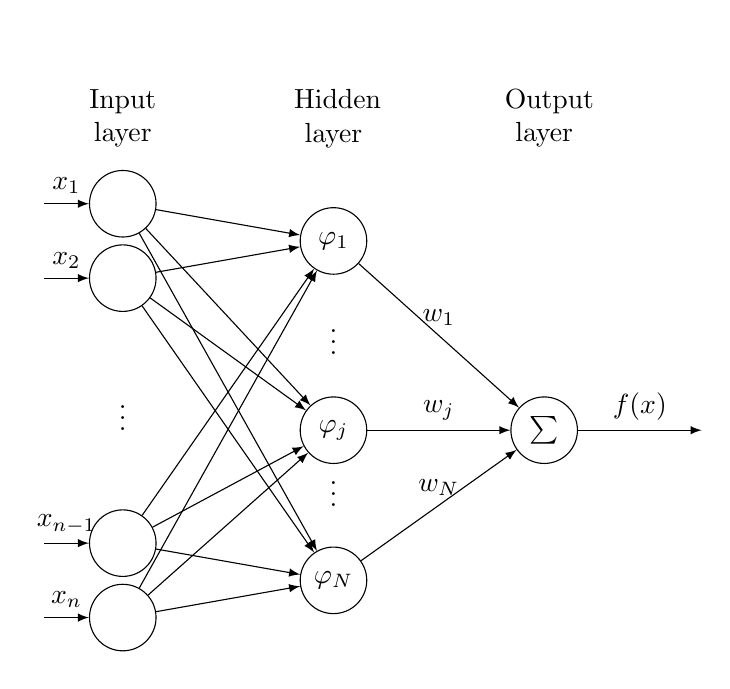
\begin{tikzpicture}[
		plain/.style={
			draw=none,
			fill=none,
		},
		net/.style={
			matrix of nodes,
			nodes={
				draw,
				circle,
				inner sep=8.5pt
			},
			nodes in empty cells,
			column sep=0.6cm,
			row sep=-11pt
		},
		>=latex
		]
		\matrix[net] (mat)
		{
			|[plain]| \parbox{1cm}{\centering Input\\layer} & 
			|[plain]| \parbox{1cm}{\centering Hidden\\layer} &
			|[plain]| \parbox{1cm}{\centering Output\\layer} \\
			& |[plain]| \\
			|[plain]| & \\
			& |[plain]| \\
			|[plain]| & |[plain]| $\vdots$\\
			|[plain]|$\vdots$& & \\
			|[plain]| & |[plain]|$\vdots$ \\
			& |[plain]| \\
			|[plain]| & \\
			& |[plain]| \\
		};
		
		
		\foreach \ai [count=\mi ]in {2,4}
		\draw[<-] (mat-\ai-1) -- node[above] {$x_\mi$} +(-1cm,0);
		\draw[<-] (mat-8-1) -- node[above] {$x_{n-1}$} +(-1cm,0);
		\draw[<-] (mat-10-1) -- node[above] {$x_{n}$} +(-1cm,0);
		
		\foreach \ai in {2,4,8,10}
		{\foreach \aii in {3,6,9}
			\draw[->] (mat-\ai-1) -- (mat-\aii-2);
		}
		
		% Final Weights
		\draw[->] (mat-3-2) --node[above]{$w_1$} (mat-6-3);
		\draw[->] (mat-6-2) --node[above]{$w_j$} (mat-6-3);
		\draw[->] (mat-9-2) --node[above]{$w_N$} (mat-6-3);
		\draw[->] (mat-6-3) -- node[above] {$f(x)$} +(2cm,0);
		
		\draw [] (mat-3-2) node(){$\varphi_1$};
		\draw [] (mat-6-2) node(){$\varphi_j$};
		\draw [] (mat-9-2) node(){$\varphi_N$};
		\draw [] (mat-6-3) node(){$\sum$};
		
		\end{tikzpicture}
		
\end{document}
	\caption{ Αρχιτεκτονική Νευρωνικού Δικτύου RBF }
	\label{fig:rbf_network_architecture}
\end{figure}

\textbf{Επίπεδο Εισόδου}: Η είσοδος ενός δικτύου RBF είναι ένα διάνυσμα $x = \begin{bmatrix} x_1,x_2, ..., x_n \end{bmatrix}^T$. Στα νευρωνικά δίκτυα αυτής της κατηγορίας το επίπεδο εισόδου είναι υπεύθυνο για την μετάδοση των επιμέρους ορισμάτων $x_i$ σε κάθε νευρώνα και όχι για κάποια περαιτέρω προεπεξεργασία δεδομένων.

\textbf{Κρυφό Επίπεδο:} Στο κρυφό επίπεδο λαμβάνει χώρο ο υπολογισμός των συναρτήσεων $\varphi_i(x)$ οι οποίες ονομάζονται \textit{συναρτήσεις βάσης} ή \textit{συναρτήσεις ενεργοποίησης}. Σε άλλους τύπους δικτύων μπορεί να υπάρχουν πάνω από ένα κρυφά επίπεδα, αλλά στα RBF δίκτυα που μελετάμε υπάρχει μόνο ένα.

Κάθε συνάρτηση βάσης είναι μια πραγματική συνάρτηση $\varphi: \mathbb{R}^n \rightarrow \mathbb{R} $, και αντιστοιχεί σε ένα σημείο του χώρου $c \in \mathbb{R}^n$. Οι συναρτήσεις $\varphi$ είναι ακτινικές συναρτήσεις, που σημαίνει πως το αποτέλεσμα τους εξαρτάται από την απόσταση της εισόδου $x$ από το σημείο $c$, ή αλλιώς μαθηματικά:
\begin{equation*}
	\varphi(x,c) = \varphi(\| x - c \|)
\end{equation*}
και από εκεί προκύπτει και η ονομασία Ακτινικά Νευρωνικά Δίκτυα. Τυπικές ακτινικές συναρτήσεις είναι η γκαουσιανή, η τετραγωνική, η αντίστροφη τετραγωνική και άλλες~\cite{wiki:rbf}, ωστόσο σε αυτήν την εργασία θα χρησιμοποιήσουμε τις γκαουσιανές συναρτήσεις οι οποίες έχουν την μορφή
\begin{equation*}
	\varphi(x) = \exp \left( - \left\| \frac{x - c}{\sigma}\right\|^2 \right)
\end{equation*}
Το σημείο $c$ ονομάζεται \textit{κέντρο} ενώ η ποσότητα $\sigma$ ονομάζεται \textit{διασπορά}. Στην εφαρμογή μας, και τα δυο αυτά μεγέθη επιλέγονται εκ των προτέρων και παραμένουν σταθερά κατά την διάρκεια των πειραμάτων. Ένα παράδειγμα μιας μονοδιάστασης γκαουσιανής συνάρτησης φαίνεται στο σχήμα $(\ref{fig:gaussian_function})$.


\textbf{Επίπεδο Εξόδου:} Η έξοδος ενός RBF νευρωνικού δικτύου είναι μια βαθμωτή συνάρτηση $f: \mathbb{R}^n \rightarrow \mathbb{R} $. Η έξοδος αυτή υπολογίζεται στο επίπεδο εξόδου ώς το σταθμισμένο άθροισμα:
\begin{equation*}
	f(x) = \sum_{i = 1}^{N} w_i \varphi_i (x)
\end{equation*}
Τα βάρη $w_i$ ονομάζονται \textit{συναπτικά βάρη}, και αποτελούν τις ελεύθερες παραμέτρους του δικτύου. Καθώς οι συναρτήσεις βάσης $\varphi_i(x)$ είναι προεπιλεγμένες και σταθερές, λέμε ότι το μοντέλο είναι \textit{γραμμικά παραμετροποιημένο} που θα πει ότι η έξοδος του είναι γραμμικός συνδυασμός των ελεύθερων παραμέτρων αυτού. Τέλος, η έξοδος του μοντέλου μπορεί να γραφτεί και διανυσματικά ώς:
\begin{equation*}
	f(x) = \begin{bmatrix} w_1 & w_2 & ... & w_n \end{bmatrix} \cdot \begin{bmatrix}
	\varphi_1(x) \\ \varphi_2(x) \\ ... \\ \varphi_n(x)
	\end{bmatrix} = 
	W^T \cdot  \varPhi(x)
\end{equation*}
Το διάνυσμα $W$ ονομάζεται \textit{διάνυσμα βαρών} ενώ το διάνυσμα $\varPhi(x)$ ονομάζεται \textit{διάνυσμα οπισθοδρομητών} στην βιβλιογραφία της αναγνώρισης συστημάτων. Η γραμμικότητα ως προς τις ελεύθερες παραμέτρους αποτελεί σημαντικό πλεονέκτημα στα προβλήματα αναγνώρισης, για αυτό και τα γραμμικά παραμετροποίημενα μοντέλα προτιμούνται σε τέτοιου είδους εφαρμογές.

\begin{figure}
	\centering
	\scalebox{.5}{% This file was created by matlab2tikz.
%
\definecolor{mycolor1}{rgb}{0.00000,0.44700,0.74100}%
%
\begin{tikzpicture}

\begin{axis}[%
width=4.521in,
height=3.566in,
at={(0.758in,0.481in)},
scale only axis,
xmin=-2,
xmax=2,
ymin=-0.1,
ymax=1.2,
axis background/.style={fill=white}
]
\addplot [color=mycolor1, line width=1.5pt, forget plot]
  table[row sep=crcr]{%
-2	0.0183156388887342\\
-1.95	0.0223149147769664\\
-1.9	0.0270518468663504\\
-1.85	0.032630755992896\\
-1.8	0.0391638950989871\\
-1.75	0.046770622383959\\
-1.7	0.0555762126114831\\
-1.65	0.0657102732275029\\
-1.6	0.0773047404432997\\
-1.55	0.0904914416636959\\
-1.5	0.105399224561864\\
-1.45	0.12215066953999\\
-1.4	0.140858420921045\\
-1.35	0.161621192465339\\
-1.3	0.184519523992989\\
-1.25	0.209611387151098\\
-1.2	0.236927758682122\\
-1.15	0.266468297813524\\
-1.1	0.298197279429887\\
-1.05	0.332039945344661\\
-1	0.367879441171442\\
-0.95	0.405554505063321\\
-0.9	0.444858066222941\\
-0.85	0.48553689515408\\
-0.8	0.527292424043049\\
-0.75	0.569782824730923\\
-0.7	0.612626394184416\\
-0.65	0.655406254326841\\
-0.6	0.697676326071031\\
-0.55	0.738968488258944\\
-0.5	0.778800783071405\\
-0.45	0.816686482598111\\
-0.4	0.852143788966211\\
-0.35	0.884705904943484\\
-0.3	0.913931185271228\\
-0.25	0.939413062813476\\
-0.2	0.960789439152323\\
-0.15	0.977751237193336\\
-0.0999999999999999	0.990049833749168\\
-0.0499999999999998	0.99750312239746\\
0	1\\
0.0499999999999998	0.99750312239746\\
0.0999999999999999	0.990049833749168\\
0.15	0.977751237193336\\
0.2	0.960789439152323\\
0.25	0.939413062813476\\
0.3	0.913931185271228\\
0.35	0.884705904943484\\
0.4	0.852143788966211\\
0.45	0.816686482598111\\
0.5	0.778800783071405\\
0.55	0.738968488258944\\
0.6	0.697676326071031\\
0.65	0.655406254326841\\
0.7	0.612626394184416\\
0.75	0.569782824730923\\
0.8	0.527292424043049\\
0.85	0.48553689515408\\
0.9	0.444858066222941\\
0.95	0.405554505063321\\
1	0.367879441171442\\
1.05	0.332039945344661\\
1.1	0.298197279429887\\
1.15	0.266468297813524\\
1.2	0.236927758682122\\
1.25	0.209611387151098\\
1.3	0.184519523992989\\
1.35	0.161621192465339\\
1.4	0.140858420921045\\
1.45	0.12215066953999\\
1.5	0.105399224561864\\
1.55	0.0904914416636959\\
1.6	0.0773047404432997\\
1.65	0.0657102732275029\\
1.7	0.0555762126114831\\
1.75	0.046770622383959\\
1.8	0.0391638950989871\\
1.85	0.032630755992896\\
1.9	0.0270518468663504\\
1.95	0.0223149147769664\\
2	0.0183156388887342\\
};
\end{axis}

\draw[<-][line width=1.2pt] (5.2,5.0) -- (5+2.615-0.35,5.0) node[right=0.0pt,scale=1.5] {$\sigma$};
\draw[->][line width=1.2pt] (5+2.615+0.35,5.0) -- (10.13,5.0);

\draw[dashed][line width=1.2pt] (7.67,5.5) -- (7.67,8.9);
\draw[dashed][line width=1.2pt] (7.67,1.18) -- (7.67,4.6);
\draw[fill=black] (7.67,8.9) circle (0.1cm)
node[anchor=south,scale=1.5] {$c$};

\end{tikzpicture}%}
	\caption{ Γκαουσιανή συνάρτηση ενεργοποίησης. Το κέντρο $c$ είναι το σημείο στο οποίο η συνάρτηση παρουσιάζει την μέγιστη τιμή, ενώ η διασπορά $\sigma$ καθορίζει τον ρυθμό που η συνάρτηση μειώνεται όσο το $x$ απομακρύνεται από το $c$. }
	\label{fig:gaussian_function}
\end{figure}


\begin{figure}
	\begin{subfigure}{0.5\textwidth}
		\includegraphics[scale=0.5]{plots/mathematicalTools/networks/components.tex}
		\caption{Επιμέρους όροι}
	\end{subfigure}
	\begin{subfigure}{0.5\textwidth}
		\includegraphics[scale=0.5]{plots/mathematicalTools/networks/f_approximation.tex}
		\caption{Συνολική Προσέγγιση}
	\end{subfigure}
	\caption{ Προσέγγιση της $f(x) = 1+x$ από ένα απλό RBF νευρωνικό δίκτυο. }
	\label{fig:rbf_approximation}
\end{figure}

\subsection{Προσεγγιστικές Ιδιότητες} \label{subsec:rbf_approximation_theorem}
Τα ακτινικά νευρωνικά δίκτυα είναι ένα πολύ χρήσιμο εργαλείο στην αναγνώριση μη γραμμικών συστημάτων. Ο λόγος είναι πως η παραπάνω δομή μπορεί να προσεγγίσει ικανοποιητικά καλά μια οποιαδήποτε συνεχή συνάρτηση όπως αναφέρεται στην ακόλουθη ιδιότητα~\cite{park1991universal}.

\textbf{Ιδιότητα Προσέγγισης:} \textit{Για κάθε συνεχή συνάρτηση $f: \mathbb{R}^n \rightarrow \mathbb{R} $ και κάθε θετική σταθερά $\epsilon > 0$ υπάρχουν ακέραιος αριθμός $q$, βέλτιστα βάρη $W^* \in \mathbb{R}^q$ και διανυσματικό πεδίο βάσης $\varPhi: \mathbb{R}^n \rightarrow \mathbb{R}^q$, τέτοια ώστε:
\begin{equation*}
	\max_{x \in \Omega_x} \left\| f(x) - W^{*T}\varPhi(x) \right\| \leq \epsilon
\end{equation*}
όπου $\Omega_x$ είναι ένα συμπαγές σύνολο προσέγγισης.
}

Σύμφωνα με την παραπάνω ιδιότητα αν το μέγεθος του διανυσματικού πεδίου βάσης $q$ είναι αρκούντως μεγάλο και οι συναρτήσεις που περιλαμβάνει είναι κατάλληλα επιλεγμένες τότε υπάρχουν βέλτιστα βάρη $W^*$ τέτοια ώστε η έξοδος του νευρωνικού δικτύου να προσεγγίζει οσοδήποτε καλά την άγνωστη συνάρτηση $f(x)$ μέσα στο σύνολο $\Omega_x$. Ως εκ τούτου, μπορούμε να αντικαταστήσουμε, χωρίς βλάβη γενικότητας, την άγνωστη συνάρτηση $f(x)$ με ένα RBF νευρωνικό δίκτυο ως εξής:
\begin{equation*}
	f(x) = W^{*T}\varPhi(x) + \epsilon_f(x)
\end{equation*}

Η ποσότητα $\epsilon_f(x)$ ονομάζεται \textit{σφάλμα μοντελοποίησης}, και εξαρτάται από την αρχιτεκτονική του νευρωνικού δικτύου, δηλαδή το πλήθος και την διάταξη των συναρτήσεων βάσης και αντίστοιχα των κέντρων και των διασπορών του νευρωνικού δικτύου.

\textbf{Παράδειγμα}\\
Στο παράδειγμα που ακολουθεί, θα γίνει μια επίδειξη των προσεγγιστικών ικανοτήτων ενός RBF νευρωνικού δικτύου. Για λόγους απλότητας θα προσεγγίσουμε την μονοδιάστατη συνάρτηση $f: \mathbb{R} \rightarrow \mathbb{R} $
\begin{equation*}
f(x) = 1+x
\end{equation*}
στο συμπαγές σύνολο $\Omega_x = [-1,1] \subset \mathbb{R}$. Για την προσέγγιση θα χρησιμοποιήσουμε ένα νευρωνικό δίκτυο RBF με τρία κέντρα κατανεμημένα στο $\Omega_x$. Τα κέντρα αυτά θα είναι τα $c = \begin{bmatrix} -0.7 & 0.0 & 0.7 \end{bmatrix}$ και η διασπορά $\sigma$ είναι $0.4$. 

{
\begin{wrapfigure}{r}{0.4\textwidth}
	\centering
	\includegraphics[scale=0.5]{plots/mathematicalTools/networks/f_approximation_dense.tex}
	\caption{Προσέγγιση με πυκνότερο δίκτυο}
	\label{fig:rbf_dense_approximation}	
\end{wrapfigure}

Τα αποτελέσματα της προσέγγισης φαίνονται στο σχήμα $(\ref{fig:rbf_approximation})$. Αρχικά στο σχήμα $(\ref{fig:rbf_approximation}.a)$ φαίνονται τα βέλτιστα βάρη για κάθε μια από τις συναρτήσεις βάσης, και το άθροισμα τους το οποίο αποτελεί την προσέγγιση $\hat{f}(x)$ φαίνεται στο σχήμα $(\ref{fig:rbf_approximation}.b)$. 

Όπως φαίνεται λοιπόν από το σχήμα $(\ref{fig:rbf_approximation}.b)$, το εκπαιδευμένο νευρωνικό δίκτυο καταφέρνει να προσεγγίσει ικανοποιητικά την άγνωστη συνάρτηση στην περιοχή ενδιαφέροντος $\Omega_x$. Το σφάλμα μοντελοποίησης $\epsilon_f(x)$ είναι η σκιαγραφημένη περιοχή, ενώ στο σχήμα φαίνεται και το μέγιστο σφάλμα $\epsilon$. Καθώς αυτό το σφάλμα είναι το ελάχιστο δυνατό για την δεδομένη αρχιτεκτονική που έχουμε επιλέξει, στην περίπτωση που απαιτείται μεγαλύτερη ακρίβεια, πρέπει να αυξήσουμε τον αριθμό των συναρτήσεων βάσης. Μια προσέγγιση με την χρήση ενός πυκνότερου δικτύου φαίνεται στο σχήμα $(\ref{fig:rbf_dense_approximation})$

}

Τέλος, είναι σημαντικό να σημειωθεί πως το θεώρημα μας εξασφαλίζει πως το σφάλμα $\epsilon_f(x)$ φράσσεται από το $\epsilon$ μόνο εντός του $\Omega_x$. Όπως φαίνεται και στο σχήμα $(\ref{fig:rbf_approximation}.b)$, όσο απομακρυνόμαστε από το $\Omega_x$ το σφάλμα μεγαλώνει ανεξέλεγκτα.


\section{Συνθήκη Επιμένουσας Διέγερσης}
Όπως είδαμε στο κεφάλαιο $2.1$, μπορούμε να χρησιμοποιήσουμε το μαθηματικό μοντέλο των νευρωνικών δικτύων $RBF$ για να προσεγγίσουμε αρκούντως καλά μια συνεχή μη-γραμμική συνάρτηση σε ένα πεδίο ενδιαφέροντος $\Omega_x$. Πώς όμως εξασφαλίζεται ότι τα βάρη $W$ θα συγκλίνουν στα βέλτιστα βάρη $W^*$ κατά την εκτίμηση παραμέτρων;

Η απάντηση στο παραπάνω ερώτημα δίνεται από την συνθήκη της επιμένουσας διέγερσης (Persistancy of Excitation Condition), η οποία δίνεται παρακάτω:

\textbf{Συνθήκη Επιμένουσας Διέγερσης:} 
\textit{Έστω $\mu$ ένα θετικό $\Sigma$-πεπερασμένο μέτρο Borel στο διάστημα $[0,\infty)$. Μια συνεχής, ομοιόμορφα φραγμένη διανυσματική συνάρτηση $\varPhi: [0,\infty) \rightarrow \mathbb{R}^q$ ικανοποιεί την συνθήκη Επιμένουσας Διέγερσης εάν υπάρχουν θετικές σταθερές $a_1$, $a_2$ και $T$ έτσι ώστε:
\begin{equation}
	a_1 \left\| W \right\|^2 
	\leq
	\int_{t_0}^{t_0 + T} \left| W^T \varPhi(\tau) \right|^2 d\mu(\tau) 
	\leq
	a_2 \left\| W \right\|^2, \quad
	\forall \: t_0 \geq 0 , \quad
	\forall \: W \in \mathbb{R}^q
	\label{eq:pe_condition}
\end{equation}
}

Διαισθητικά το παραπάνω θεώρημα θα πει πως η συνθήκη επιμένουσας διέγερσης ικανοποιείται όταν η τροχιά του συστήματος εξερευνεί πλήρως τον χώρο ελεύθερων παραμέτρων. Η παρακάτω έννοια θα εξηγηθεί και στην συνέχεια με παραδείγματα.

\textbf{Παρατήρηση 1:} Στην παραπάνω εξίσωση, οι σταθερές $a_1$ και $a_2$ ονομάζονται επίπεδα διέγερσης, και οι τιμές τους είναι καθοριστικές για την απόδοση των αλγορίθμων αναγνώρισης (ρυθμός σύγκλισης, άνω φράγματα σφαλμάτων). Ωστόσο, το παραπάνω Θεώρημα είναι θεώρημα ύπαρξης αυτών των τιμών, και όχι υπολογισμού τους.

\textbf{Παρατήρηση 2:} Ο λόγος που το διάνυσμα οπισθοδρομητών $\varPhi(x)$ εμφανίζεται στην παραπάνω εξίσωση ως συνάρτηση του χρόνου $t$ είναι επειδή στην πράξη, το διάνυσμα καταστάσεων $x(t)$ είναι μια καμπύλη $x: [0,\infty) \rightarrow \mathbb{R}^n$. Η ικανοποίηση της ΣΕΔ στις εφαρμογές \textit{οnline} αναγνώρισης συστημάτων ανάγεται ακριβώς στο πρόβλημα της σχεδίασης ενός ελεγκτή που επιτυγχάνει την παρακολούθηση μιας τροχιάς η οποία διεγείρει επαρκώς την δυναμική συστήματος.

\textbf{Παρατήρηση 3:} Η ισχύς του παραπάνω θεωρήματος είναι γενική και δεν ισχύει μόνο για το μοντέλο των RBF νευρωνικών δικτύων. Εν αντιθέσει, το θεώρημα δεν θέτει κανέναν περιορισμό για την δομή του διανύσματος οπισθοδρομητών $varPhi(\tau)$, συνεπώς οποιαδήποτε επιλογή μοντέλου και σετ δεδομένων $x(t)$ μπορούν να χρησιμοποιηθούν.

\textbf{Παρατήρηση 4:} Είναι σημαντικό να τονίσουμε πως η ΣΕΔ το μόνο που εξασφαλίζει είναι ότι τα βέλτιστα βάρη για το επιλεγμένο μοντέλο μπορούν να βρεθούν. Αυτό δεν συνεπάγεται απαραίτητα ότι το μοντέλο αυτό είναι ικανό να προσεγγίσει επαρκώς την δυναμική του συστήματος (Παράδειγμα 2).

\subsection{Παράδειγμα 1: Μη ικανοποίηση της Σ.Ε.Δ}
Έστω ότι θέλουμε να προσεγγίσουμε την άγνωστη συνάρτηση $f(x) = \sqrt{x}$ στο κλειστό σύνολο $\Omega_x = [0,2]$. Για τον σκοπό αυτό, θα χρησιμοποιήσουμε δυο συναρτήσεις ράμπα τοποθετημένες στο $x=0$ και στο $x=1$. Καθώς η συνάρτηση ράμπα περιγράφεται από τον παρακάτω τύπο
\begin{equation*}
	R_i(x) = \begin{cases}
	x-i \:&, x \geq i\\
	0 \: &, x<i 
	\end{cases}
\end{equation*}
το μαθηματικό μοντέλο που χρησιμοποιούμε είναι το:
\begin{equation}
y = a R_0(x) + b R_1(x)
\label{eq:ramp_model}
\end{equation}
όπου $a$ και $b$ οι ελεύθεροι παράμετροι. Χρησιμοποιώντας αυτό το μοντέλο, η βέλτιστη δυνατή προσέγγιση φαίνεται στο σχήμα $(\ref{fig:sqrt_approximation})$.

\begin{figure}
	\centering
	\scalebox{1}{\documentclass{article}
\usepackage{pgfplots}
\usepgfplotslibrary{fillbetween}
\pgfplotsset{compat=newest}
\usepackage{tikz}
\usetikzlibrary{calc,arrows}
\usetikzlibrary{fadings}

\begin{document}
	
	\definecolor{blue_mat}{rgb}{0.00000,0.44700,0.74100}%
	\definecolor{orange_mat}{rgb}{0.85000,0.32500,0.09800}%
	
	\begin{tikzpicture}
	\begin{axis}[
	axis lines=middle,
	clip=false,
	ymin=-0.1,
	xmin=-0.1,
	xmax=3,
	xtick = {0,1,2,3},
	xlabel = {$x$},
	ylabel = {$y$},
	yticklabels=\empty,
	%legend pos=north west,
	legend style={at={(0.05,0.97)}, anchor=north west, legend cell align=left, align=left, draw=white!15!black},
	every axis x label/.style={
		at={(ticklabel* cs:1.02)},
		anchor=west,
	},
	every axis y label/.style={
		at={(ticklabel* cs:1.01)},
		anchor=south
	},
	]
	\begin{scope}
	\shade[top color=yellow,bottom color=white,opacity=0.3]
	(0.0,0.0) rectangle (1,-0.3);
	\shade[top color=blue,bottom color=white,opacity=0.1]
	(1.0,0.0) rectangle (2,-0.3);
	\end{scope}
	\node at (0.5,-0.15) {$\Omega_1$};
	\node at (1.5,-0.15) {$\Omega_2$};
	
	\addplot+[color=blue_mat,mark=none,samples=200,domain=0.001:2.0,line width=1.2pt, name path = A] {sqrt(x)};
	\addlegendentry{$f(x)$}
	\addplot+[color=orange_mat,mark=none,samples=200,domain=0.001:1,line width=1.2pt,] {1.1090*x};
	\addlegendentry{$\hat{f}(x)$}
	\addplot+[color=orange_mat,mark=none,samples=200,domain=1:2.0,line width=1.2pt, name path = B] {-0.8445*(x-1) + 1.1090*x};
	
	\addplot+[dashed,color=blue_mat,mark=none,samples=200,domain=2.0:2.5,line width=1.2pt] {sqrt(x)};
	
	\addplot+[dashed,color=orange_mat,mark=none,samples=200,domain=2.0:2.5,line width=1.2pt] {-0.8445*(x-1) + 1.1090*x};
	
	\draw[dashed] (1,0) -- (1,1.1090);
	\draw[dashed] (2,0) -- (2,2*1.1090-0.8445);
	
	\addplot [gray!30] fill between [of=A and B];
	
	
	\end{axis}

	
	\end{tikzpicture}
	
\end{document}}
	\caption{ Προσέγγιση της $\sqrt{x}$ από ράμπες}
	\label{fig:sqrt_approximation}
\end{figure}

\subsubsection{Διαισθητική Ερμηνεία}
Με την φράση \emph{"η τροχιά του συστήματος εξερευνεί πλήρως τον χώρο ελεύθερων παραμέτρων"} εννοούμε πως κατά την διάρκεια συλλογής δεδομένων, ανεξαρτήτως του αν ο αλγόριθμος είναι online ή offline, πρέπει η τροχιά $x(t)$ να διεγείρει όλες τις συνιστώσες του διανύσματος του διανύσματος οπισθοδρομητών.

Στο συγκεκριμένο παράδειγμα, το διάνυσμα οπισθοδρομητών είναι το
\begin{equation*}
	\varPhi(x(t)) = \begin{bmatrix}
	R_0(x(t)) \\ R_1(x(t)) 
	\end{bmatrix}
\end{equation*}
Εάν κατά την διάρκεια εκτέλεσης ενός πειράματος αναγνώρισης, η τροχιά $x(t)$ ανήκει εξολοκλήρου στο σύνολο $\Omega_1$ (σχήμα ...), τότε η εκτίμηση $\hat{f}(x)$ εκφυλίζεται σε:
\begin{equation*}
\begin{split}
\hat{f}(x) &=\begin{bmatrix} a & b \end{bmatrix} 
\begin{bmatrix} R_0(x) \\ R_1(x) \end{bmatrix} \xRightarrow{x \in \Omega_1}\\
&= a R_0(x)
\end{split}
\end{equation*}
και κατά συνέπεια η παράμετρος $b$ δεν επηρεάζει καθόλου το αποτέλεσμα. Συνεπώς, κανένας αλγόριθμος εκτίμησης παραμέτρων δεν μπορεί να εκτιμήσει σωστά αυτή την παράμετρο με αποτέλεσμα την αποτυχία του πειράματος αναγνώρισης.


\begin{figure}
	\centering
	\scalebox{1}{\documentclass{article}
\usepackage{pgfplots}
\usepgfplotslibrary{fillbetween}
\pgfplotsset{compat=newest}
\usepackage{tikz}
\usetikzlibrary{calc,arrows}
\usetikzlibrary{fadings}
\usepackage{amsmath}
\usepackage{amssymb}

\begin{document}
	
	\definecolor{blue_mat}{rgb}{0.00000,0.44700,0.74100}%
	\definecolor{orange_mat}{rgb}{0.85000,0.32500,0.09800}%
	
	\begin{tikzpicture}
	\begin{axis}[
	axis lines=middle,
	clip=false,
	ymin=-0.1,
	ymax=1.4,
	xmin=-0.1,
	xmax=2.5,
	xtick = {0},
	ytick={0},
	%yticklabel,={0,1,2},
	xlabel = {$\varphi_1(x)$},
	ylabel = {$\varphi_2(x)$},
	axis equal,
	%legend pos=north west,
	%legend style={at={(0.05,0.97)}, anchor=north west, legend cell %align=left, align=left, draw=white!15!black},
%	every axis x label/.style={
%		at={(ticklabel* cs:1.02)},
%		anchor=west,
%	},
%	every axis y label/.style={
%		at={(ticklabel* cs:1.05)},
%		anchor=south
%	},
	]
	\begin{scope}
	\shade[top color=yellow,bottom color=white,opacity=0.3]
	(0.0,0.0) rectangle (1,-0.3);
	\shade[top color=blue,bottom color=white,opacity=0.1]
	(1.0,0.0) rectangle (2,-0.3);
	\end{scope}
	\node at (0.5,-0.15) {$\Omega_1$};
	\node at (1.5,-0.15) {$\Omega_2$};
	
	
	\addplot+[color=orange,mark=none,samples=200,domain=0.001:1.0,line width=1.8pt, name path = A] {0};
	\addplot+[color=blue_mat,mark=none,samples=200,domain=1.001:2.0,line width=1.5pt, name path = B] {x-1};
	
	\draw[dashed] (0,1) -- (2,1);
	\draw[dashed] (2,0) -- (2,1);
	
	\draw[line width = 0.8] (0,0) circle (1);
	
	\draw[->,color = black,opacity = 0.1, line width = 0.7,>=latex] (0,0) -- (0.5,0);
	\draw[->,color = black,opacity = 0.2, line width = 0.7,>=latex] (0,0) -- (1,0);
	\draw[->,color = black,opacity = 0.4, line width = 0.7,>=latex] (0,0) -- (0.5,0);
	\draw[->,color = black,opacity = 0.45, line width = 0.7,>=latex] (0,0) -- (1.25,0.25);
	\draw[->,color = black,opacity = 0.5, line width = 0.7,>=latex] (0,0) -- (1.5,0.5);
	\draw[->,color = black,opacity = 0.6, line width = 0.7,>=latex] (0,0) -- (1.75,0.75);
	\draw[->,color = black,opacity = 0.7, line width = 0.7,>=latex] (0,0) -- (2,1);
	
	\node at (0.0,1.0) [anchor=south east]{$1$};
	\node at (1.0,0.0) [anchor=north west]{$1$};
	\node at (2.0,0.0) [anchor=north west]{$2$};
	
	\node at (2.0,1.0) [anchor=west]{$\varPhi(x)$};
	
	\pgfmathsetmacro{\a}{60}
	\draw[->,color = black,opacity = 1, line width = 0.7,>=latex] (0,0) --
	({cos(\a)},{sin(\a)}) node[above=0.1cm,midway] {$c$};
	
%	\addplot+[color=blue_mat,mark=none,samples=200,domain=0.001:2.0,line width=1.2pt, name path = A] {sqrt(x)};
%	\addlegendentry{$f(x)$}
%	\addplot+[color=orange_mat,mark=none,samples=200,domain=0.001:1,line width=1.2pt,] {1.1090*x};
%	\addlegendentry{$\hat{f}(x)$}
%	\addplot+[color=orange_mat,mark=none,samples=200,domain=1:2.0,line width=1.2pt, name path = B] {-0.8445*(x-1) + 1.1090*x};
%	
%	\addplot+[dashed,color=blue_mat,mark=none,samples=200,domain=2.0:2.5,line width=1.2pt] {sqrt(x)};
%	
%	\addplot+[dashed,color=orange_mat,mark=none,samples=200,domain=2.0:2.5,line width=1.2pt] {-0.8445*(x-1) + 1.1090*x};
%	
%	\draw[dashed] (1,0) -- (1,1.1090);
%	\draw[dashed] (2,0) -- (2,2*1.1090-0.8445);
%	
%	\addplot [gray!30] fill between [of=A and B];
	
	
	\end{axis}

	
	\end{tikzpicture}
	
\end{document}}
	\caption{ Γεωμετρικός τόπος του $\varPhi(x)$ στο $\Omega$}
	\label{fig:regressor_locus}
\end{figure}

\subsubsection{Μαθηματική Απόδειξη}
Αρχικά, ας εξετάσουμε την σχέση $(\ref{eq:pe_condition})$. Χρησιμοποιώντας τον γεωμετρικό ορισμό του εσωτερικού γινομένου για τον όρο $W^T \varPhi(x(t))$ έχουμε
\begin{equation*}
\begin{split}
a_1 \left\| W \right\|^2  &\leq
\int_{t_0}^{t_0 + T} \left| W^T \varPhi(\tau) \right|^2 d\mu(\tau) 
\leq
a_2 \left\| W \right\|^2
\xRightarrow{a^T \cdot b = \| a\| \|b \| \cos{\theta}}\\
% Second Line
a_1  \cancel{\left\| W \right\|^2} &\leq % left
\cancel{\left\| W \right\|^2}  
\int_{t_0}^{t_0 + T} \left\| \varPhi(\tau) \right\|^2 \cos^2(\theta) d\mu(\tau) \leq % middle
a_2 \cancel{\left\| W \right\|^2} \Rightarrow \\ %right
a_1 &\leq
\int_{t_0}^{t_0 + T} \left\| \varPhi(\tau) \right\|^2 \cos^2(\theta) d\mu(\tau)
\leq a_2, \quad \text{όπου} \: \theta = \angle (W, \varPhi(\tau))
\end{split}
\end{equation*}
Καθώς το διάνυσμα $W \in \mathbb{R}^q$, η γωνία $\theta$ της παραπάνω εξίσωσης πρακτικά είναι η γωνία του διανύσματος οπισθοδρομητών $\varPhi(x(t))$ με οποιοδήποτε μοναδιαίο διάνυσμα $c$ στον χώρο $\mathbb{R}^q$. Συνεπώς, η παραπάνω σχέση γράφεται αλλιώς και ως:
\begin{equation}
	a_1 \leq \int_{t_0}^{t_0 + T} \left\| c^T \varPhi(\tau) \right\|^2 d\mu(\tau)
	\leq a_2, \quad
	\forall \: t_0 \geq 0 , \quad
	\| c \| = 1
	\label{eq:pe_alternative}
\end{equation}
για κάθε μοναδιαίο διάνυσμα του χώρου $\mathbb{R}^q$. Η εξίσωση $(\ref{eq:pe_alternative})$ αποτελεί μια ισοδύναμη έκφραση της Συνθήκης επιμένουσας διέγερσης, η οποία σε αυτό το παράδειγμα διευκολύνει την ανάλυση.

Επιστρέφοντας στο παράδειγμα μας, έστω ότι έχουμε βρει έναν μηχανισμό ελέγχου που εξαναγκάζει την τροχιά $x(t)$ του συστήματος να εκτελέσει την περιοδική κίνηση
\begin{equation*}
x(t) = 0.5(1+\cos(t))
\end{equation*}
, συνεπώς $ 0 \leq x(t) \leq 1$ άρα $x(t) \in \Omega_1$.

Καθώς η συνάρτηση $x(t)$ είναι περιοδική με περίοδο $2\pi$, έτσι και η συνάρτηση $c^T \varPhi(x(t))$ της εξίσωσης $(\ref{eq:pe_alternative})$, ως σύνθεση με περιοδική συνάρτηση είναι επίσης περιοδική. Έτσι, επιλέγοντας στο θεώρημα ... την σταθερά $T$ ίση με την περίοδο, μπορούμε να χρησιμοποιήσουμε την παρακάτω ιδιότητα των περιοδικών συναρτήσεων:
\begin{equation*}
	\int_{a}^{a+T} f(x) dx = \int_{0}^{T} f(x) dx
\end{equation*}
για να απλοποιήσουμε περαιτέρω το ολοκλήρωμα της ΣΕΔ ως εξής:
\begin{equation*}
\int_{t_0}^{t_0 + T} \left| c^T \varPhi(x(\tau)) \right|^2 d\tau = 
\int_{0}^{T} \left| c^T \varPhi(x(\tau)) \right|^2 d\tau, \quad \forall t_0
\end{equation*}
Από την παραπάνω σχέση, είναι ευκολότερο να αντιληφθεί κανείς την φυσική σημασία της ΣΕΔ. Πρέπει, κατά μήκος μιας περιόδου το διάνυσμα $\varPhi(x(t))$ να εξερευνεί κάθε κατεύθυνση $c$ του χώρου ελεύθερων παραμέτρων. Όσο πιο αποτελεσματική είναι η διέγερση αυτή, τότε τόσο αυξάνεται το κάτω φράγμα $a_1$ το οποίο ονομάζεται και \textit{επίπεδο διέγερσης}.

Για να επιδείξουμε το παραπάνω συμπέρασμα, στο σχήμα $(\ref{fig:regressor_locus})$ μελετάμε την γεωμετρική συμπεριφορά του διανύσματος $\varPhi(x(t))$ συναρτήσει της τροχιάς $x(t)$. Καθότι έχουμε συναρτήσεις ράμπας, το διάνυσμα γράφεται ώς:
\begin{equation*}
	\varPhi(x) = 
	\begin{cases}
	[x, 0]^T    &, \: x \in \Omega_1\\
	[x,x-1]^T &, \: x \in \Omega_2\\
	\end{cases}
\end{equation*}
Όταν η τροχιά $x(t) \in \Omega_1$, τότε το διάνυσμα $\varPhi$ κινείται πάνω στο πορτοκαλί ευθύγραμμο τμήμα. Σε αυτή την περίπτωση όμως, είναι πάντα κάθετο στο μοναδιαίο διάνυσμα $c = [ 1 \: 0 ]^T$, συνεπώς το εσωτερικό γινόμενο $c^T \varPhi(x(\tau))$ είναι $0$ καθ'όλη την διάρκεια της περιόδου. 

Μέσω αυτού του αντιπαραδείγματος βλέπουμε πως δεν υπάρχει θετικό $a_1$ που να ικανοποιεί την παρακάτω σχέση.
\begin{equation*}
	0 < a_1 \leq \int_{0}^{T} \left| c^T \varPhi(x(\tau)) \right|^2 d\tau \quad
	\forall c \in
	\{c \mid c \in \mathbb{R}^2, \: \|c\| =1 \}
\end{equation*}
συνεπώς η διανυσματική συνάρτηση $\varPhi$ δεν ικανοποιεί την συνθήκη επιμένουσας διέγερσης.

Αντιθέτως, μέσω του σχήματος $(\ref{fig:regressor_locus})$ βλέπουμε πως εάν επιλέξουμε μια τροχιά $x(t)$ που να επισκέπτεται και τα δύο σύνολα $\Omega_1$ και $\Omega_2$, τότε το διάνυσμα $\varPhi$ κινείται πάνω στα δύο ευθύγραμμα τμήματα (πορτοκαλί και μπλέ). Σε αυτή την περίπτωση δεν υπάρχει διάνυσμα $c$ του μοναδιαίου κύκλου που να είναι κάθετο σε όλη την διάρκεια της περιόδου $T$, συνεπώς ικανοποιείται η συνθήκη επιμένουσας διέγερσης.

Παρόλα αυτά, ακόμα και σε αυτό το απλό παράδειγμα είναι αρκετά δύσκολος ο αναλυτικός υπολογισμός του επιπέδου διέγερσης $a_1$.

\subsection{Παράδειγμα 2: Σ.Ε.Δ και ποιότητα εκτίμησης}
Σε αυτό το δεύτερο παράδειγμα το ζητούμενο μας είναι η προσέγγιση της άγνωστης συνάρτησης $f(x) = 1 + 0.3\cos(5x)$ με την χρήση του μοντέλου
\begin{equation*}
	y = a \cos(x) + b \sin(x)
\end{equation*}

Όπως και πριν, έτσι και εδώ θα υποθέσουμε πως έχουμε βρει έναν μηχανισμό ελέγχου που εξαναγκάζει την τροχιά $x(t)$ του συστήματος να εκτελέσει την κίνηση $x(t) = t$. Παρόλο που η κίνηση δεν είναι περιοδική όπως πριν, αυτό δεν αποτελεί πρόβλημα αφού τόσο η άγνωστη συνάρτηση $f$, όσο και το διάνυσμα οπισθοδρομητών $\varPhi$ είναι περιοδικές συναρτήσεις του χρόνου.

\subsubsection{Μαθηματική Ανάλυση}
Ας εξετάσουμε την ΣΕΔ για το συγκεκριμένο παράδειγμα χρησιμοποιώντας τον ορισμό $(\ref{eq:pe_alternative})$. Ομοίως με πριν, το διάνυσμα οπισθοδρομητών είναι περιοδικό με περίοδο $2\pi$, συνεπώς ο υπολογισμός της ΣΕΔ ανάγεται στην μελέτη του ολοκληρώματος
\begin{equation*}
	\int_{0}^{T} \left| c^T \varPhi(x(\tau)) \right|^2 d\tau
	\forall c \in
	\{c \mid c \in \mathbb{R}^2, \: \|c\| =1 \}
\end{equation*}

Αναλύοντας το εσωτερικό γινόμενο $c^T \varPhi(x(\tau))$ περαιτέρω, προκύπτει
\begin{equation}
\int_{0}^{T} \left| c^T \varPhi(x(\tau)) \right|^2 d\tau = 
\int_{0}^{T} \|c\|^2 \| \varPhi(x(\tau)) \|^2 \cos^2(\theta) d\tau, \quad
\text{όπου} \: \theta = \angle (c, \varPhi(\tau))
%\forall c \in
%\{c \mid c \in \mathbb{R}^2, \: \|c\| =1 \}
\label{eq:pe_sines}
\end{equation}
Καθώς όμως, το $c$ είναι μοναδιαίο, το μέτρο του είναι $1$. Επίσης, το διάνυσμα οπισθοδρομητών είναι το
\begin{equation*}
	\varPhi(x) = \begin{bmatrix} \cos(x) \\ \sin(x) \end{bmatrix}
\end{equation*}
το μέτρο  $\| \varPhi(x(\tau)) \|$ είναι επίσης $1$ για κάθε $x$. Συνεπώς το ολοκλήρωμα της σχέσης $(\ref{eq:pe_sines})$ απλοποιείται ακόμα περισσότερο και τελικά καταλήγουμε στην τελική μορφή:
\begin{equation*}
	\int_{0}^{T}\cos^2(\theta(t)) d\tau
\end{equation*}
{
\begin{wrapfigure}{r}{0.4\textwidth}
	\centering
	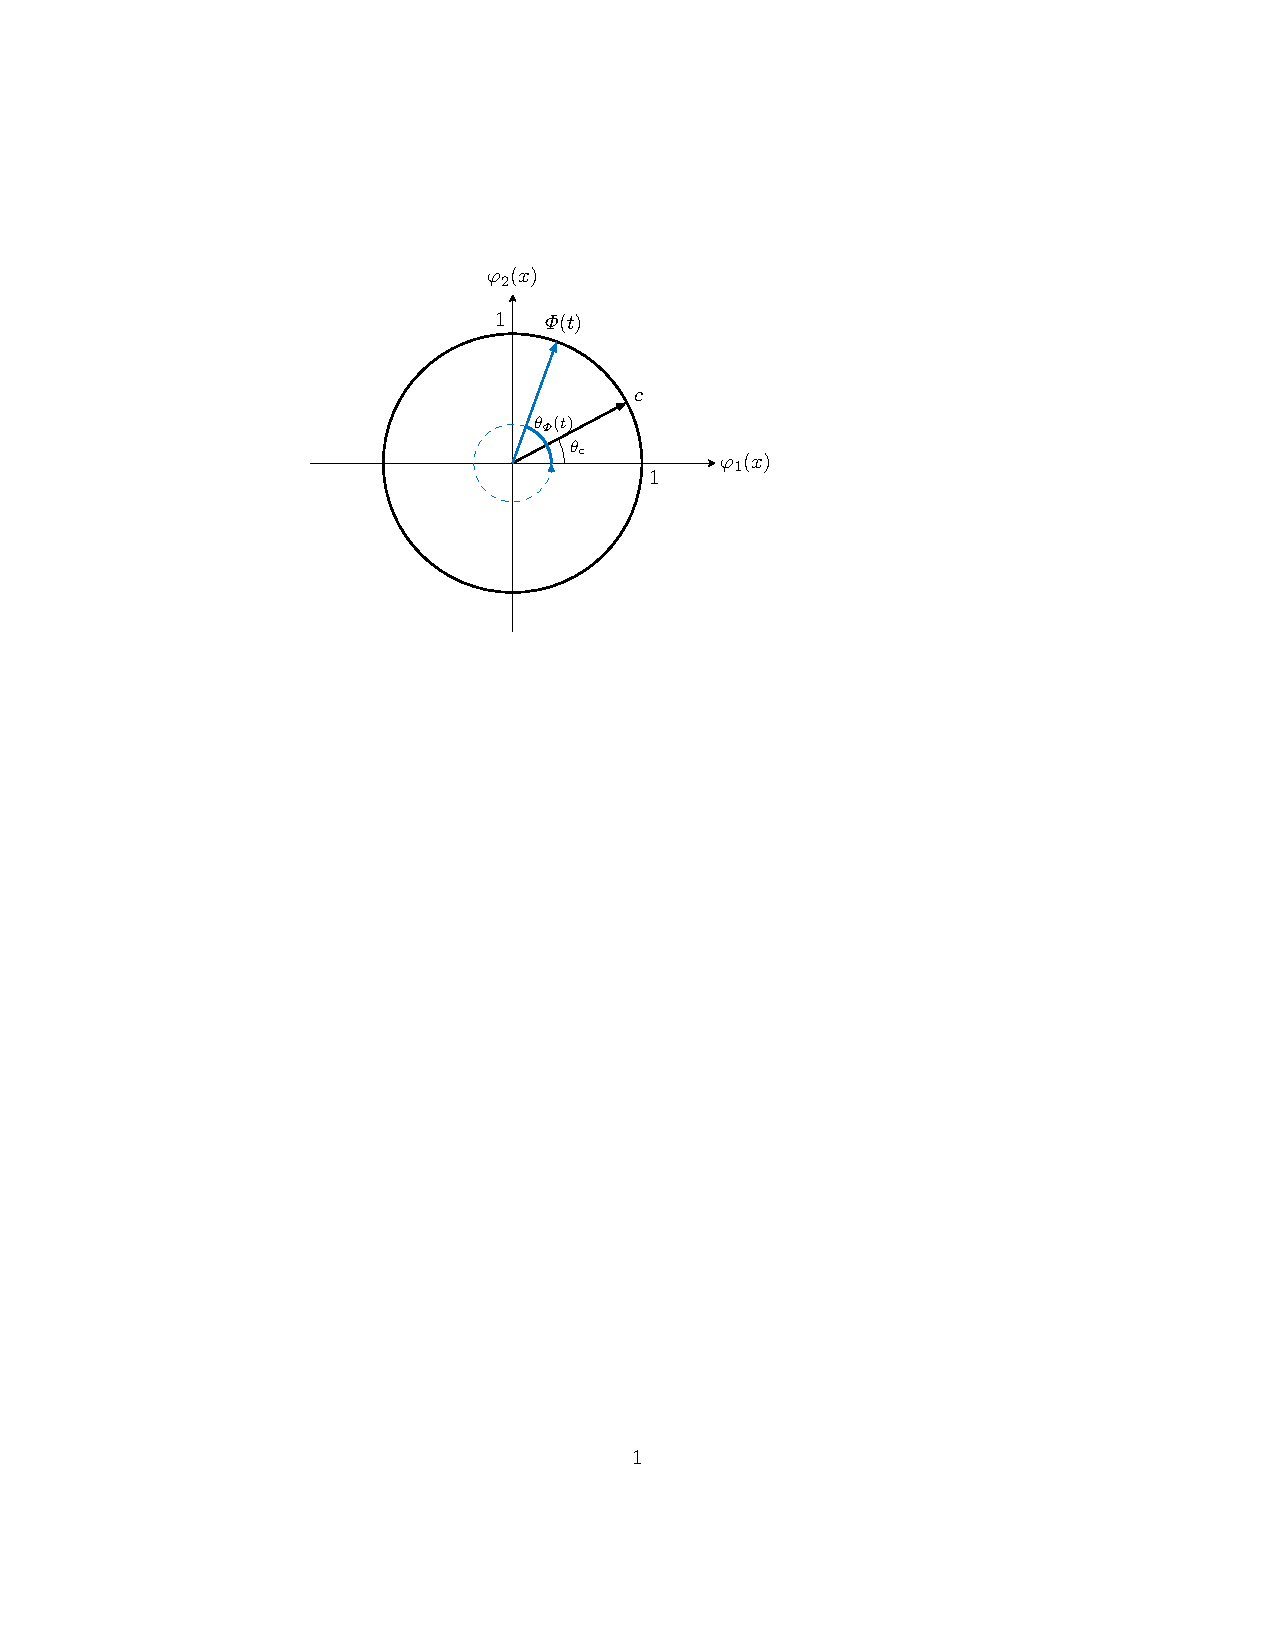
\includegraphics[scale=0.8]{plots/mathematicalTools/pe/regressors_sine.tex}
	\caption{}
	\label{fig:regressors_theta}	
\end{wrapfigure}
όπου η γωνία $\theta(t)$ δίνεται από την σχέση
\begin{equation*}
	\theta(t) = \theta_{\varPhi}(t) - \theta_c ,
	\quad \theta_c \in [0,2\pi]
\end{equation*}
με τα $\theta_{\varPhi}$ και $\theta_c$ να φαίνονται στο σχήμα $(\ref{fig:regressors_theta})$. Λόγω της συμμετρίας του σχήματος, το αποτέλεσμα θα είναι το ίδιο για κάθε γωνία $\theta_c$, και συνεπώς η αριθμητική τιμή του ολοκληρώματος της ΣΕΔ είναι τελικά
\begin{equation*}
\int_{0}^{2\pi}\cos^2(\tau) d\tau = \pi = a_1 = a_2
\end{equation*}

Όπως μπορούμε να δούμε η απλότητα του παραδείγματος μας επιτρέπει τον ακριβή υπολογισμό των επιπέδων διέγερσης και ως εκ τούτου την μαθηματική επαλήθευση της ΣΕΔ.

}

Παρόλα αυτά, χρησιμοποιώντας το παραπάνω μοντέλο για να προσεγγίσουμε την άγνωστη $f(x)$ στο πεδίο ενδιαφέροντος, καταλήγουμε στην προσέγγιση του σχήματος $(\ref{fig:sines_approximation})$ η οποία δεν είναι ιδιαίτερα ικανοποιητική.

\begin{figure}[h!]
\centering
\scalebox{.6}{% This file was created by matlab2tikz.
%
\definecolor{mycolor1}{rgb}{0.00000,0.44700,0.74100}%
\definecolor{mycolor2}{rgb}{0.85000,0.32500,0.09800}%
%
\begin{tikzpicture}

\begin{axis}[%
width=0.571\textwidth,
height=0.4\textwidth,
at={(0\textwidth,0\textwidth)},
scale only axis,
xmin=0,
xmax=3,
ymin=0,
ymax=1.5,
axis background/.style={fill=white},
legend style={legend cell align=left, align=left, draw=white!15!black}
]
\addplot [name path = A,color=mycolor1, line width=1.2pt]
  table[row sep=crcr]{%
0	1.3\\
0.01	1.29962507811849\\
0.02	1.29850124958341\\
0.03	1.29663132338081\\
0.04	1.29401997335237\\
0.05	1.29067372651319\\
0.06	1.28660094673768\\
0.07	1.28181181385421\\
0.08	1.27631829820087\\
0.09	1.2701341307058\\
0.1	1.26327476856711\\
0.11	1.25575735661785\\
0.12	1.2476006844729\\
0.13	1.23882513956472\\
0.14	1.22945265618535\\
0.15	1.21950666066215\\
0.16	1.20901201280415\\
0.17	1.19799494376549\\
0.18	1.1864829904812\\
0.19	1.17450492683916\\
0.2	1.16209069176044\\
0.21	1.14927131436752\\
0.22	1.13607883642767\\
0.23	1.12254623226525\\
0.24	1.108707326343\\
0.25	1.09459670871858\\
0.26	1.08024964858738\\
0.27	1.06570200612791\\
0.28	1.05099014287007\\
0.29	1.03615083081021\\
0.3	1.02122116050031\\
0.31	1.00623844834093\\
0.32	0.991240143309613\\
0.33	0.97626373335798\\
0.34	0.961346651711343\\
0.35	0.946526183305152\\
0.36	0.931839371592074\\
0.37	0.917322925952646\\
0.38	0.903013129940949\\
0.39	0.888945750594614\\
0.4	0.875155949035857\\
0.41	0.861678192586986\\
0.42	0.848546168620043\\
0.43	0.835792700355919\\
0.44	0.823449664823396\\
0.45	0.811547913183178\\
0.46	0.800117193616053\\
0.47	0.789186076967934\\
0.48	0.778781885337626\\
0.49	0.768930623785808\\
0.5	0.75965691533592\\
0.51	0.750983939429433\\
0.52	0.742933373989316\\
0.53	0.735525341236514\\
0.54	0.728778357394882\\
0.55	0.722709286410261\\
0.56	0.717333297799402\\
0.57	0.712663828734073\\
0.58	0.708712550455123\\
0.59	0.705489339100464\\
0.6	0.703002251019866\\
0.61	0.701257502638282\\
0.62	0.700259454918016\\
0.63	0.700010602458597\\
0.64	0.700511567261574\\
0.65	0.701761097175836\\
0.66	0.703756069027341\\
0.67	0.70649149642542\\
0.68	0.709960542226162\\
0.69	0.714154535621709\\
0.7	0.719062993812761\\
0.71	0.724673648210117\\
0.72	0.730972475099756\\
0.73	0.737943730694819\\
0.74	0.745569990486878\\
0.75	0.753832192798132\\
0.76	0.762709686425675\\
0.77	0.772180282258748\\
0.78	0.782220308739958\\
0.79	0.792804671031848\\
0.8	0.803906913740916\\
0.81	0.815499287042328\\
0.82	0.827552816040019\\
0.83	0.840037373188854\\
0.84	0.85292175359779\\
0.85	0.866173753025862\\
0.86	0.879760248376007\\
0.87	0.89364728048556\\
0.88	0.907800139006474\\
0.89	0.922183449163112\\
0.9	0.936761260170766\\
0.91	0.951497135093894\\
0.92	0.966354241919484\\
0.93	0.981295445617902\\
0.94	0.996283400961133\\
0.95	1.01128064586639\\
0.96	1.02624969503183\\
0.97	1.04115313363027\\
0.98	1.05595371082677\\
0.99	1.07061443288634\\
1	1.08509865563897\\
1.01	1.09937017607103\\
1.02	1.11339332281389\\
1.03	1.12713304530383\\
1.04	1.14055500139011\\
1.05	1.15362564317255\\
1.06	1.16631230085375\\
1.07	1.17858326439658\\
1.08	1.19040786278279\\
1.09	1.20175654067454\\
1.1	1.21260093228738\\
1.11	1.22291393228992\\
1.12	1.23266976355308\\
1.13	1.24184404157941\\
1.14	1.25041383545175\\
1.15	1.25835772514846\\
1.16	1.2656558550824\\
1.17	1.27228998372952\\
1.18	1.27824352922321\\
1.19	1.28350161080027\\
1.2	1.28805108599511\\
1.21	1.29188058348907\\
1.22	1.29498053153278\\
1.23	1.29734318187054\\
1.24	1.29896262910697\\
1.25	1.29983482546735\\
1.26	1.29995759091502\\
1.27	1.29933061860031\\
1.28	1.29795547562746\\
1.29	1.29583559913775\\
1.3	1.29297628771841\\
1.31	1.28938468815887\\
1.32	1.28506977758756\\
1.33	1.28004234103375\\
1.34	1.2743149444706\\
1.35	1.26790190340672\\
1.36	1.26081924710495\\
1.37	1.25308467851745\\
1.38	1.24471753003761\\
1.39	1.2357387151791\\
1.4	1.22617067630299\\
1.41	1.21603732852354\\
1.42	1.20536399993284\\
1.43	1.19417736829382\\
1.44	1.18250539435968\\
1.45	1.17037725198661\\
1.46	1.15782325521433\\
1.47	1.14487478249678\\
1.48	1.13156419827232\\
1.49	1.11792477206948\\
1.5	1.10399059535051\\
1.51	1.08979649630041\\
1.52	1.07537795277468\\
1.53	1.06077100362308\\
1.54	1.04601215861136\\
1.55	1.03113830716578\\
1.56	1.01618662616879\\
1.57	1.00119448703622\\
1.58	0.986199362308139\\
1.59	0.971238731987051\\
1.6	0.956349989857416\\
1.61	0.941570350020652\\
1.62	0.926936753879263\\
1.63	0.912485777802573\\
1.64	0.89825354170485\\
1.65	0.884275618764333\\
1.66	0.870586946508814\\
1.67	0.857221739490007\\
1.68	0.844213403764994\\
1.69	0.831594453398479\\
1.7	0.819396429194553\\
1.71	0.80764981986112\\
1.72	0.796383985803996\\
1.73	0.785627085741192\\
1.74	0.77540600632078\\
1.75	0.765746294918275\\
1.76	0.756672095781503\\
1.77	0.748206089682555\\
1.78	0.740369437227666\\
1.79	0.733181725966726\\
1.8	0.726660921434597\\
1.81	0.720823322246641\\
1.82	0.715683519360666\\
1.83	0.711254359607129\\
1.84	0.707546913578751\\
1.85	0.704570447959803\\
1.86	0.702332402364219\\
1.87	0.700838370740436\\
1.88	0.700092087389438\\
1.89	0.700095417630945\\
1.9	0.700848353141087\\
1.91	0.70234901197321\\
1.92	0.704593643261762\\
1.93	0.707576636597503\\
1.94	0.711290536050607\\
1.95	0.715726058806602\\
1.96	0.720872118368574\\
1.97	0.726715852267634\\
1.98	0.733242654212392\\
1.99	0.740436210597078\\
2	0.748278541277064\\
};
\addlegendentry{$f(x)$}

\addplot [name path = B,color=mycolor2, line width=1.2pt]
  table[row sep=crcr]{%
0	0.716430833556827\\
0.01	0.725518964887895\\
0.02	0.734534544927072\\
0.03	0.743476672123865\\
0.04	0.752344452273009\\
0.05	0.761136998603876\\
0.06	0.769853431869162\\
0.07	0.778492880432804\\
0.08	0.787054480357144\\
0.09	0.795537375489324\\
0.1	0.803940717546902\\
0.11	0.812263666202673\\
0.12	0.820505389168708\\
0.13	0.828665062279579\\
0.14	0.836741869574773\\
0.15	0.844735003380292\\
0.16	0.852643664389417\\
0.17	0.860467061742637\\
0.18	0.868204413106737\\
0.19	0.875854944753026\\
0.2	0.883417891634718\\
0.21	0.890892497463424\\
0.22	0.898278014784793\\
0.23	0.905573705053245\\
0.24	0.912778838705835\\
0.25	0.9198926952352\\
0.26	0.926914563261616\\
0.27	0.933843740604133\\
0.28	0.94067953435079\\
0.29	0.947421260927908\\
0.3	0.954068246168449\\
0.31	0.960619825379427\\
0.32	0.967075343408381\\
0.33	0.973434154708888\\
0.34	0.979695623405116\\
0.35	0.985859123355415\\
0.36	0.991924038214923\\
0.37	0.997889761497212\\
0.38	1.00375569663492\\
0.39	1.00952125703943\\
0.4	1.0151858661595\\
0.41	1.02074895753894\\
0.42	1.02620997487324\\
0.43	1.03156837206523\\
0.44	1.03682361327965\\
0.45	1.04197517299676\\
0.46	1.04702253606488\\
0.47	1.05196519775191\\
0.48	1.0568026637958\\
0.49	1.06153445045397\\
0.5	1.06616008455171\\
0.51	1.07067910352946\\
0.52	1.07509105548908\\
0.53	1.07939549923907\\
0.54	1.08359200433862\\
0.55	1.08768015114072\\
0.56	1.09165953083411\\
0.57	1.09552974548413\\
0.58	1.09929040807254\\
0.59	1.10294114253622\\
0.6	1.10648158380475\\
0.61	1.10991137783697\\
0.62	1.11323018165633\\
0.63	1.11643766338522\\
0.64	1.11953350227812\\
0.65	1.12251738875374\\
0.66	1.12538902442591\\
0.67	1.12814812213347\\
0.68	1.13079440596892\\
0.69	1.13332761130611\\
0.7	1.1357474848266\\
0.71	1.13805378454506\\
0.72	1.14024627983345\\
0.73	1.14232475144405\\
0.74	1.14428899153144\\
0.75	1.14613880367325\\
0.76	1.14787400288981\\
0.77	1.14949441566263\\
0.78	1.1509998799518\\
0.79	1.15239024521213\\
0.8	1.15366537240827\\
0.81	1.15482513402855\\
0.82	1.15586941409777\\
0.83	1.15679810818881\\
0.84	1.15761112343303\\
0.85	1.15830837852957\\
0.86	1.15888980375352\\
0.87	1.15935534096283\\
0.88	1.15970494360417\\
0.89	1.15993857671756\\
0.9	1.1600562169399\\
0.91	1.16005785250725\\
0.92	1.15994348325606\\
0.93	1.15971312062317\\
0.94	1.15936678764463\\
0.95	1.15890451895347\\
0.96	1.15832636077617\\
0.97	1.15763237092805\\
0.98	1.15682261880753\\
0.99	1.15589718538915\\
1	1.15485616321547\\
1.01	1.15369965638785\\
1.02	1.152427780556\\
1.03	1.15104066290645\\
1.04	1.1495384421498\\
1.05	1.14792126850689\\
1.06	1.14618930369372\\
1.07	1.14434272090534\\
1.08	1.14238170479849\\
1.09	1.14030645147313\\
1.1	1.13811716845288\\
1.11	1.13581407466422\\
1.12	1.13339740041459\\
1.13	1.13086738736942\\
1.14	1.1282242885279\\
1.15	1.12546836819771\\
1.16	1.12259990196859\\
1.17	1.11961917668476\\
1.18	1.11652649041628\\
1.19	1.1133221524292\\
1.2	1.11000648315464\\
1.21	1.10657981415676\\
1.22	1.10304248809962\\
1.23	1.09939485871286\\
1.24	1.09563729075639\\
1.25	1.09177015998388\\
1.26	1.08779385310517\\
1.27	1.08370876774764\\
1.28	1.07951531241643\\
1.29	1.07521390645357\\
1.3	1.07080497999607\\
1.31	1.0662889739329\\
1.32	1.06166633986092\\
1.33	1.05693754003966\\
1.34	1.05210304734518\\
1.35	1.04716334522272\\
1.36	1.04211892763837\\
1.37	1.03697029902968\\
1.38	1.03171797425523\\
1.39	1.02636247854311\\
1.4	1.02090434743844\\
1.41	1.01534412674978\\
1.42	1.00968237249456\\
1.43	1.00391965084349\\
1.44	0.99805653806393\\
1.45	0.992093620462276\\
1.46	0.986031494325318\\
1.47	0.979870765860618\\
1.48	0.973612051135887\\
1.49	0.967255976017384\\
1.5	0.960803176107323\\
1.51	0.954254296680318\\
1.52	0.947609992618855\\
1.53	0.940870928347802\\
1.54	0.93403777776797\\
1.55	0.927111224188724\\
1.56	0.920091960259649\\
1.57	0.912980687901289\\
1.58	0.905778118234953\\
1.59	0.898484971511607\\
1.6	0.891101977039845\\
1.61	0.88362987311296\\
1.62	0.876069406935121\\
1.63	0.868421334546643\\
1.64	0.860686420748393\\
1.65	0.852865439025304\\
1.66	0.844959171469031\\
1.67	0.836968408699742\\
1.68	0.828893949787054\\
1.69	0.82073660217013\\
1.7	0.812497181576934\\
1.71	0.804176511942659\\
1.72	0.795775425327335\\
1.73	0.787294761832622\\
1.74	0.778735369517802\\
1.75	0.770098104314975\\
1.76	0.761383829943462\\
1.77	0.75259341782344\\
1.78	0.743727746988794\\
1.79	0.73478770399922\\
1.8	0.725774182851568\\
1.81	0.71668808489044\\
1.82	0.707530318718061\\
1.83	0.698301800103417\\
1.84	0.689003451890679\\
1.85	0.679636203906919\\
1.86	0.670200992869131\\
1.87	0.660698762290554\\
1.88	0.651130462386329\\
1.89	0.641497049978472\\
1.9	0.631799488400196\\
1.91	0.622038747399579\\
1.92	0.612215803042584\\
1.93	0.602331637615465\\
1.94	0.592387239526524\\
1.95	0.582383603207286\\
1.96	0.572321729013045\\
1.97	0.562202623122835\\
1.98	0.552027297438814\\
1.99	0.541796769485071\\
2	0.531512062305874\\
};
\addlegendentry{$\hat{f}(x)$}

\addplot [color=mycolor1, dashed, line width=1.2pt, forget plot]
  table[row sep=crcr]{%
2.01	0.756750044509856\\
2.02	0.765829545949245\\
2.03	0.775494351570146\\
2.04	0.78572030439184\\
2.05	0.796481844857846\\
2.06	0.807752074721502\\
2.07	0.819502824277569\\
2.08	0.831704722771831\\
2.09	0.844327271812677\\
2.1	0.857338921601202\\
2.11	0.87070714978927\\
2.12	0.884398542768452\\
2.13	0.898378879186635\\
2.14	0.912613215483597\\
2.15	0.927065973231691\\
2.16	0.9417010280634\\
2.17	0.956481799963431\\
2.18	0.971371344699714\\
2.19	0.986332446164733\\
2.2	1.00132770939642\\
2.21	1.01631965404606\\
2.22	1.03127080805971\\
2.23	1.04614380133873\\
2.24	1.06090145914563\\
2.25	1.07550689502153\\
2.26	1.0899236029831\\
2.27	1.10411554876853\\
2.28	1.11804725990437\\
2.29	1.13168391436827\\
2.3	1.1449914276259\\
2.31	1.15793653782455\\
2.32	1.17048688893039\\
2.33	1.18261111160177\\
2.34	1.19427890159616\\
2.35	1.20546109551507\\
2.36	1.21612974369725\\
2.37	1.22625818007839\\
2.38	1.23582108884231\\
2.39	1.24479456769738\\
2.4	1.25315618761975\\
2.41	1.26088504891426\\
2.42	1.2679618334528\\
2.43	1.27436885295953\\
2.44	1.28009009322239\\
2.45	1.2851112541203\\
2.46	1.28941978536598\\
2.47	1.29300491787516\\
2.48	1.29585769068366\\
2.49	1.29797097334516\\
2.5	1.29933948375357\\
2.51	1.2999598013456\\
2.52	1.2998303756503\\
2.53	1.29895153016452\\
2.54	1.29732546154428\\
2.55	1.29495623411428\\
2.56	1.29184976970923\\
2.57	1.28801383287233\\
2.58	1.28345801144796\\
2.59	1.27819369261704\\
2.6	1.27223403443506\\
2.61	1.26559393294373\\
2.62	1.25828998493869\\
2.63	1.25034044648613\\
2.64	1.24176518729213\\
2.65	1.23258564103879\\
2.66	1.2228247518111\\
2.67	1.21250691674878\\
2.68	1.20165792506604\\
2.69	1.19030489359206\\
2.7	1.17847619899297\\
2.71	1.166201406845\\
2.72	1.15351119773595\\
2.73	1.14043729057963\\
2.74	1.1270123633352\\
2.75	1.11326997132919\\
2.76	1.09924446338471\\
2.77	1.0849708959673\\
2.78	1.07048494556195\\
2.79	1.05582281950054\\
2.8	1.04102116546235\\
2.81	1.02611697987391\\
2.82	1.01114751543725\\
2.83	0.996150188017505\\
2.84	0.981162483122775\\
2.85	0.966221862209849\\
2.86	0.951365669050085\\
2.87	0.936631036389425\\
2.88	0.922054793135874\\
2.89	0.907673372306403\\
2.9	0.893522719963389\\
2.91	0.87963820536817\\
2.92	0.86605453257632\\
2.93	0.852805653695579\\
2.94	0.839924684023265\\
2.95	0.827443819275279\\
2.96	0.815394255113584\\
2.97	0.803806109173291\\
2.98	0.792708345784262\\
2.99	0.782128703575366\\
3	0.772093626142354\\
};
\addplot [color=mycolor2, dashed, line width=1.2pt, forget plot]
  table[row sep=crcr]{%
2.01	0.521174204363373\\
2.02	0.510784229434745\\
2.03	0.500343176508826\\
2.04	0.489852089682208\\
2.05	0.47931201805483\\
2.06	0.468724015625071\\
2.07	0.458089141184353\\
2.08	0.447408458211255\\
2.09	0.436683034765176\\
2.1	0.425913943379521\\
2.11	0.415102260954456\\
2.12	0.404249068649212\\
2.13	0.393355451773977\\
2.14	0.382422499681359\\
2.15	0.371451305657458\\
2.16	0.360442966812532\\
2.17	0.349398583971294\\
2.18	0.338319261562823\\
2.19	0.327206107510127\\
2.2	0.316060233119351\\
2.21	0.304882752968646\\
2.22	0.293674784796712\\
2.23	0.282437449391026\\
2.24	0.271171870475765\\
2.25	0.259879174599433\\
2.26	0.248560491022206\\
2.27	0.23721695160301\\
2.28	0.225849690686333\\
2.29	0.214459844988795\\
2.3	0.203048553485475\\
2.31	0.191616957296012\\
2.32	0.1801661995705\\
2.33	0.168697425375169\\
2.34	0.157211781577881\\
2.35	0.145710416733445\\
2.36	0.134194480968761\\
2.37	0.122665125867807\\
2.38	0.111123504356488\\
2.39	0.0995707705873353\\
2.4	0.0880080798241\\
2.41	0.0764365883262214\\
2.42	0.0648574532332076\\
2.43	0.0532718324489183\\
2.44	0.0416808845257766\\
2.45	0.0300857685489163\\
2.46	0.0184876440202728\\
2.47	0.00688767074263386\\
2.48	-0.0047129912963404\\
2.49	-0.0163131820401123\\
2.5	-0.027911741479274\\
2.51	-0.0395075097675476\\
2.52	-0.0510993273377676\\
2.53	-0.062686035017836\\
2.54	-0.0742664741466412\\
2.55	-0.08583948668992\\
2.56	-0.0974039153560629\\
2.57	-0.108958603711839\\
2.58	-0.120502396298043\\
2.59	-0.132034138745036\\
2.6	-0.143552677888182\\
2.61	-0.155056861883166\\
2.62	-0.166545540321176\\
2.63	-0.17801756434394\\
2.64	-0.189471786758618\\
2.65	-0.200907062152513\\
2.66	-0.212322247007614\\
2.67	-0.223716199814949\\
2.68	-0.235087781188733\\
2.69	-0.246435853980303\\
2.7	-0.257759283391838\\
2.71	-0.269056937089832\\
2.72	-0.28032768531833\\
2.73	-0.291570401011903\\
2.74	-0.302783959908349\\
2.75	-0.313967240661123\\
2.76	-0.325119124951469\\
2.77	-0.336238497600252\\
2.78	-0.347324246679473\\
2.79	-0.358375263623462\\
2.8	-0.369390443339733\\
2.81	-0.380368684319495\\
2.82	-0.391308888747798\\
2.83	-0.402209962613315\\
2.84	-0.413070815817745\\
2.85	-0.423890362284818\\
2.86	-0.434667520068903\\
2.87	-0.445401211463203\\
2.88	-0.456090363107523\\
2.89	-0.466733906095607\\
2.9	-0.477330776082024\\
2.91	-0.487879913388608\\
2.92	-0.498380263110418\\
2.93	-0.508830775221232\\
2.94	-0.519230404678549\\
2.95	-0.529578111528088\\
2.96	-0.539872861007788\\
2.97	-0.55011362365128\\
2.98	-0.560299375390833\\
2.99	-0.570429097659762\\
3	-0.580501777494281\\
};
\addplot [gray!30] fill between [of=A and B];
\end{axis}
\end{tikzpicture}%}
\caption{ Προσέγγιση της $f(x)$ του Παραδείγματος $2$. }
\label{fig:sines_approximation}
\end{figure}

\pagebreak
Το συμπέρασμα που προσπαθούμε να καταλήξουμε μέσω αυτού του παραδείγματος είναι πως ακόμα και αν η ΣΕΔ ικανοποιείται, αυτό δεν συνεπάγεται υποχρεωτικά στην επιτυχία της εφαρμογής αναγνώρισης. Πρέπει και το μοντέλο που χρησιμοποιείται να είναι ικανό να προσεγγίσει την ικανοποιητικά την άγνωστη συνάρτηση.

\subsection{ΣΕΔ για RBF νευρωνικά δίκτυα} \label{subsec:rbf_PE}
Όπως είδαμε, η μαθηματική εξασφάλιση της ικανοποίησης της Συνθήκης Επιμένουσας Διέγερσης είναι αρκετά πολύπλοκη, ακόμα και σε πολύ απλές εφαρμογές όπως αυτές των Παραδειγμάτων $1$ και $2$. 

Καθώς στην εργασία αυτή χρησιμοποιούμε ως μοντέλα τα RBF νευρωνικά δίκτυα, σε αυτό το κεφάλαιο παρουσιάζουμε ένα αποτέλεσμα που μας επιτρέπει να εγγυηθούμε την ικανοποίηση της ΣΕΔ σε ένα τόσο σύνθετο πρόβλημα.

\textbf{Θεώρημα:} 
Έστω το σύνολο $I = [t_0, t_0 + T]$, όπου $t_0$ και $T$
θετικές σταθερές, και τα σύνολα $I_i = \{ t \in I :  \| x(t) - c_i \| \} \leq \epsilon, \: i = 1,\dots, q $ με το $\epsilon \leq \frac{1}{2} \min_{i \neq j} \{\| c_i - c_j \| \}$. Εάν υπάρχει σταθερά $T$ έτσι ώστε τα μέτρα $\mu(I_i)$ να είναι κάτω φραγμένο από μια σταθερά $\tau_0$ που είναι ανεξάρτητη του $t_0$ και του $i$, τότε το διάνυσμα οπισθοδρομητών $\varPhi(x(t))$ ικανοποιεί την συνθήκη επιμένουσας διέγερσης της εξίσωσης $(\ref{eq:pe_condition})$.

\subsubsection{Φυσική Σημασία}
Η ερμηνεία του παραπάνω θεωρήματος είναι η εξής: Εάν εντός μιας περιόδου $T$, για κάθε κέντρο $c_i$ υπάρχει ένα χρονικό διάστημα $I_i$ στο οποίο η τροχιά $x(t)$ διέρχεται αρκούντως κοντά από αυτό, και ο χρόνος $\mu (I_i)$ που παραμένει αρκούντως κοντά είναι πάντα μεγαλύτερος από μια σταθερά $\tau_0$, τότε το διανυσματικό πεδίο $\varPhi(x(t))$ ικανοποιεί την ΣΕΔ της εξίσωσης $(\ref{eq:pe_condition})$.

Με αυτόν τον τρόπο, κάθε συνάρτηση ενεργοποίησης $\varphi_i(x(t))$ φτάνει κοντά στην μέγιστη τιμή της τουλάχιστον μια φορά εντός κάθε περιόδου, διεγείροντας έτσι την αντίστοιχη μοναδιαία κατεύθυνση $c$ του χώρου ελεύθερων παραμέτρων $\mathbb{R}^q$.

ίσως μπορώ να βαλω ενα σχήμα εδω... (will see)

\section{Έλεγχος Προδιαγεγραμμένης Απόκρισης} \label{sec:ppc_introduction}
Ο Έλεγχος Προδιαγεγραμμένης Απόκρισης (Prescribed Performance Control) είναι μια μεθοδολογία ελέγχου που μας επιτρέπει να ελέγξουμε ένα συνεχές δυναμικό σύστημα, εφόσον αυτό ικανοποιεί κάποιες συνθήκες που θα διατυπωθούν παρακάτω. Το μεγάλο πλεονέκτημα αυτής της μεθοδολογίας είναι ότι εγγυάται πως το σφάλμα παρακολούθησης εξόδου θα συγκλίνει σε μια προαποφασισμένη και οσοδήποτε μικρή περιοχή του μηδενός με προεπιλεγμένη ταχύτητα και υπερύψωση.

Ο έλεγχος Προδιαγεγραμμένης Απόκρισης εισήχθη στην εργασία~\cite{bechlioulis2008robust} το 2008, και τα τελευταία χρόνια έχει αναπτυχθεί εκτεταμένα. Παρόλο που στις εργασίες αυτές έχουν αναπτυχθεί πολλές παραλλαγές που να εξασφαλίζουν προδιαγεγραμμένη απόκριση εξόδου σε strict feedback συστήματα~\cite{bechlioulis2009adaptive}, pure feedback συστήματα~\cite{bechlioulis2014low} και άλλα, σε αυτό το κεφάλαιο θα παρουσιάσουμε την βασική ιδέα της μεθόδου. Στο κεφάλαιο 3 θα εμβαθύνουμε παρουσιάζοντας έναν συγκεκριμένο τρόπο εφαρμογής της που να εξυπηρετεί τις ανάγκες του προβλήματος μας, και θα αποδείξουμε μαθηματικά την ορθότητα του.

\subsection{Ορισμός του προβλήματος}
Έστω ένα γενικό μη γραμμικό σύστημα της μορφής 
\begin{equation}
\begin{split}
\dot{x} &= f(x,u,t) \\
y &= h(x)
\end{split}
\label{eq:general_nonlinear_sys}
\end{equation}
όπου $x \in \mathbb{R}^n$ το διάνυσμα καταστάσεων, $ u\in \mathbb{R}^m$ το διάνυσμα εισόδων ελέγχου και $y \in \mathbb{R}^p$ είναι η έξοδος του συστήματος. Τα διανυσματικά πεδία $f: \mathbb{R}^n \times \mathbb{R}^m \times \mathbb{R}^+ \rightarrow \mathbb{R}^n$ και $h:\mathbb{R}^n \rightarrow \mathbb{R}^p$ είναι τοπικά Lipschitz συνεχή στα ορίσματά τους. Έστω επίσης και η αρκούντως ομαλή και φραγμένη τροχιά παρακολούθησης
\begin{equation*}
	y_d(t) = \begin{bmatrix}
		y_{d1}(t) & y_{d2}(t) & \cdots & y_{dp}(t)
	\end{bmatrix}^T
\end{equation*}
καθώς και τα αντίστοιχα σφάλματα εξόδου:
\begin{equation*}
	e_i(t) = y_i(t) - y_{di}(t), \quad i = 1,\dots ,p
\end{equation*}
Αυτό που επιδιώκουμε είναι η σύγκλιση των σφαλμάτων $e_i$ σε μια προαποφασισμένη και οσοδήποτε μικρή περιοχή του μηδενός με προεπιλεγμένη ταχύτητα σύγκλισης και υπερύψωση.

Το πρώτο βήμα είναι η μαθηματική περιγραφή των εννοιών αυτών. Για τον σκοπό αυτό ορίζουμε τις συναρτήσεις επίδοσης:

\textbf{Συνάρτηση Επίδοσης:} Μια συνάρτηση $\rho: \mathbb{R}^+ \rightarrow \mathbb{R}^+$ καλείται συνάρτηση επίδοσης εάν είναι φραγμένη, θετική, γνησίως φθίνουσα και ικανοποιεί τη σχέση:
\begin{equation*}
	\lim\limits_{t \rightarrow \infty} \rho(t) > 0
\end{equation*} 

Μια τυπική επιλογή συνάρτησης συμμετοχής είναι η συνάρτηση
\begin{equation}
	\rho(t) = ( \rho_0 - \rho_{\infty} ) e^{-\lambda t} + \rho_{\infty}
	\label{eq:exp_perf}
\end{equation}
Ο λόγος είναι πως η παραπάνω επιλογή μας επιτρέπει να διαμορφώσουμε το σφάλμα σταθερής κατάστασης επιλέγοντας το $\rho_{\infty}$, το αρχικό σφάλμα επιλέγοντας το $\rho_0$ και τον ρυθμό σύγκλισης επιλέγοντας το $\lambda$.

Στην συνέχεια, για να μοντελοποιήσουμε την υπερύψωση, ορίζουμε τους αριθμούς $\overline{M}_i$ και $\barbelow{M}_i$ ώς
\begin{equation}
	(\barbelow{M}_i, \overline{M}_i) = 
	\begin{cases}
	(-M_i ,1) \quad &\text{όταν} \quad e_i(0) > 0 \\
	(-1 ,M_i) \quad &\text{όταν} \quad e_i(0) < 0 
	\end{cases}
	\quad i = 1,\dots ,p
	\label{eq:ppc_overshoot}
\end{equation}
και το συνολικό πρόβλημα της Προδιαγεγραμμένης Απόκρισης Εξόδου (ΠΑΕ) περιγράφεται από τις εξισώσεις:
\begin{equation}
	\barbelow{M}_i \rho_i(t) < e_i(t) < \overline{M}_i \rho_i(t),
	\: \forall t \geq 0, \: i = 1,\dots ,p
	\label{eq:prescibred_performance}
\end{equation}

\pagebreak

\begin{figure}[h!]
	\centering
	\tikzstyle{every node}=[font=\normalsize]
\pgfplotsset{every tick/.style={draw=none}}

\begin{tikzpicture}
\begin{axis}[%
    width=350.0,
    height=130.0,
    at={(0,500)},
    scale only axis,
    xmin=0,
    xmax=5,
    ymin=-1.3,
    ymax=3.1,
    ylabel style={font=\color{white!15!black}},
    xtick = \empty,
    ytick = {-1.05, -0.175, 0.5, 2.1, 3},
    yticklabels = {$-M_i\rho_{i0}$, $-M_i\rho_{i\infty}$, $\rho_{i\infty}$, $e_i(0)$, $\rho_{i0}$},
    axis background/.style={fill=white},
    legend style={legend cell align=left, align=left, draw=white!15!black},
    xlabel style={font=\normalsize},ylabel style={font=\normalsize},ticklabel style={font=\normalsize},x tick label style={font=\normalsize},y tick label style={font=\normalsize},legend style={font=\normalsize}
]
\addplot [black, name path = A, dashed, domain=0.001:4.999, samples=101] {(3 - 0.5)*exp(-1.5*x) + 0.5};
\addplot [black, name path = B, dashed, domain=0.001:4.999, samples=101] {-0.35*((3 - 0.5)*exp(-1.5*x) + 0.5)};
\addplot [black, smooth] coordinates {(0,2.1) (0.3,-0.4) (1.5,0.5) (3.5,0.1) (5,0.1)};
\addplot [black, dotted] coordinates {(0,0.5) (5,0.5)};
\addplot [black, dotted] coordinates {(0,-0.175) (5,-0.175)};
\addplot [gray!30] fill between [of=A and B];
\node [] at (axis cs: 0.3,1) {$e_i(t)$};
\node [] at (axis cs: 0.6,2.3) {$\rho_i(t)$};
\node [] at (axis cs: 0.8,-0.95) {$-M_i \rho_i(t)$};

\node [] at (axis cs: 4.6,-1.0) {$e_i(0) > 0$};
\end{axis}

\begin{axis}[%
width=350.0,
height=130.0,
at={(0,0)},
scale only axis,
xmin=0,
xmax=5,
ymax=1.3,
ymin=-3.1,
ylabel style={font=\color{white!15!black}},
xlabel = {Time, $t$},
xtick = \empty,
ytick = {1.05, 0.175, -0.5, -2.1, -3},
yticklabels = {$M_i\rho_{i0}$, $M_i\rho_{i \infty}$, $-\rho_{i \infty}$, $e_i(0)$, $-\rho_{i0}$},
axis background/.style={fill=white},
legend style={legend cell align=left, align=left, draw=white!15!black},
xlabel style={font=\normalsize},ylabel style={font=\normalsize},ticklabel style={font=\normalsize},x tick label style={font=\normalsize},y tick label style={font=\normalsize},legend style={font=\normalsize}
]
\addplot [black, name path = A, dashed, domain=0.001:4.999, samples=101] {-(3 - 0.5)*exp(-1.5*x) - 0.5};
\addplot [black, name path = B, dashed, domain=0.001:4.999, samples=101] {0.35*((3 - 0.5)*exp(-1.5*x) + 0.5)};
\addplot [black, smooth] coordinates {(0,-2.1) (0.3,0.4) (1.5,-0.5) (3.5,-0.1) (5,-0.1)};
\addplot [black, dotted] coordinates {(0,-0.5) (5,-0.5)};
\addplot [black, dotted] coordinates {(0,0.175) (5,0.175)};
\addplot [gray!30] fill between [of=A and B];
\node [] at (axis cs: 0.3,-1) {$e_i(t)$};
\node [] at (axis cs: 0.6,-2.3) {$-\rho_i(t)$};
\node [] at (axis cs: 0.8,0.95) {$M_i \rho_i(t)$};

\node [] at (axis cs: 4.6,-2.8) {$e_i(0 ) <0$};
\end{axis}
\end{tikzpicture}

	\caption{Μαθηματική περιγραφή της Προδιαγεγραμμένης Απόκρισης}
	\label{fig:ppc_illustration}
\end{figure}


Η ανίσωση $(\ref{eq:prescibred_performance})$ περιγράφεται σχηματικά στην γραφική παράσταση $(\ref{fig:ppc_illustration})$. Όπως μπορούμε να δούμε το πλάτος της τελικής ζώνης σύγκλισης καθορίζεται από την σταθερά $\rho_{i \infty}$ της εξίσωσης $(\ref{eq:exp_perf})$ ενώ ο ρυθμός σύγκλισης σε αυτή την ζώνη από την αντίστοιχη σταθερά $\lambda_i$. 

Ο λόγος που τα όρια $\overline{M}_i$ και $\barbelow{M}_i$ καθορίζονται με βάση την εξίσωση $(\ref{eq:ppc_overshoot})$ είναι επειδή όταν το αρχικό σφάλμα $e_i$ είναι θετικό, περιμένουμε υπερύψωση στα αρνητικά και αντίστοιχα στα θετικά στην περίπτωση που το $e_i$ είναι αρνητικό. Πολλαπλασιάζοντας και τα δύο άκρα με την σταθερά $M_i$ το μόνο που επιτυγχάνεται είναι η κλιμάκωση (scale) της συνάρτησης επίδοσης, ενώ χρησιμοποιώντας την εξίσωση $(\ref{eq:ppc_overshoot})$ μπορούμε να επιβάλουμε μέγιστη υπερύψωση ίση με $M_i \rho_{i0}$. Μάλιστα, εάν επιλέξουμε $M_i = 0$ είναι εφικτή και η περιγραφή της μηδενικής υπερύψωσης.

Τέλος, είναι πολύ σημαντικό να τονίσουμε πως για να ισχύει η εξίσωση $(\ref{eq:prescibred_performance})$ για κάθε $t \geq 0$ πρέπει η τιμή $\rho_{i0}$ να είναι μεγαλύτερη από το αρχικό πλάτος του αρχικού σφάλματος $| e_{i}(0) |$ αλλιώς για $t = 0$ το σφάλμα βρίσκεται έξω από την ζώνη.

Με βάση τα παραπάνω λοιπόν, το πρόβλημα της Προδιαγεγραμμένης Απόκρισης Εξόδου (ΠΑΕ) ορίζεται ώς εξής: 
\pagebreak


\textbf{Πρόβλημα ΠΑΕ:}
\textit{ Να σχεδιαστεί μια συνεχής είσοδος ελέγχου $u$ για το σύστημα $(\ref{eq:general_nonlinear_sys})$ έτσι ώστε όλα τα σήματα κλειστού βρόχου να διατηρούνται φραγμένα και τα σφάλματα εξόδου $e_i(t), \: i = 1,\dots ,p$ να ικανοποιούν τις σχέσεις:
\begin{equation}
	\barbelow{M}_i' \rho_i(t) \leq e_i(t) \leq \overline{M}_i'  \rho_i(t),
	\: \forall t \geq 0, \: i = 1,\dots ,p
	\label{eq:ppc_problem_definition}
\end{equation}
για κάποιες σταθερές $\barbelow{M}_i'$ και $\overline{M}_i'$ για τις οποίες ισχύουν:
\begin{equation*}
	\barbelow{M}_i < \barbelow{M}_i' \leq \overline{M}_i' < \overline{M}_i, \: i = 1,\dots ,p
\end{equation*}
με τα $\barbelow{M}_i$ και $\overline{M}_i$ να ορίζονται από την σχέση $(\ref{eq:ppc_overshoot})$ και $\rho_i(t), \: i = 1,\dots ,p$ κατάλληλα επιλεγμένες συναρτήσεις επίδοσης.
}

\subsection{Μετασχηματισμός σε πρόβλημα σταθεροποίησης}
Καθώς το πρόβλημα ΠΑΕ στην μορφή της εξίσωσης $(\ref{eq:ppc_problem_definition})$ είναι αρκετά δύσκολο να αντιμετωπιστεί, παρακάτω θα παρουσιαστεί ένας μετασχηματισμός των σφαλμάτων εξόδου, ο οποίος τα διαμορφώνει αναφορικά με τα χαρακτηριστικά απόκρισης της εξίσωσης $(\ref{eq:prescibred_performance})$ με σκοπό την διευκόλυνση της ανάλυσης. Ο μετασχηματισμός αυτός έχει την μορφή:
\begin{equation}
	\varepsilon_i(t) = T_i \left( \frac{e_i(t)}{\rho_i(t)} \right)
	, \: i = 1,\dots ,p
	\label{eq:ppc_trasformation_error}
\end{equation}
όπου οι ποσότητες $\varepsilon_i(t)$ ονομάζονται μετασχηματισμένα σφάλματα, και οι συναρτήσεις μετασχηματισμού $T_i(\cdot)$ είναι θετικές, γνησίως αύξουσες που ορίζουν απεικονίσεις της μορφής:
\begin{equation*}
	T_i: \left( \barbelow{M}_i, \overline{M}_i\right) \rightarrow 
	(- \infty, \infty), \: i = 1,\dots ,p
\end{equation*}
όπου τα $\barbelow{M}_i$ και  $\overline{M}_i$ δίνονται από την εξίσωση $(\ref{eq:ppc_overshoot})$. Η ποσότητα $e_i(t)/\rho_i(t)$ ονομάζεται αλλιώς και κανονικοποιημένο σφάλμα, και συμβολίζεται ώς $\xi_i(t)$.

Μια τέτοια συνάρτηση μετασχηματισμού είναι η
\begin{equation}
	T_i \left( \frac{e_i(t)}{\rho_i(t)} \right) = T_i \left( \xi_i(t) \right) =
	\ln \left( \frac{-\barbelow{M}_i + \xi_i(t) }{\overline{M}_i - \xi_i(t)} \right)
	\label{eq:ppc_log_transform}
\end{equation}
η οποία αναπαρίσταται γραφικά και στο σχήμα $(\ref{fig:ppc_transformation_function})$. Χρησιμοποιώντας αυτό το εργαλείο, μπορούμε να επαναπροσδιορίσουμε το πρόβλημα της ΠΑΕ χρησιμοποιώντας την ακόλουθη πρόταση:

\textbf{Ισοδύναμο Πρόβλημα ΠΑΕ:}
\textit{ Εάν τα μετασχηματισμένα σφάλματα $\varepsilon_i(t), \: i = 1,\dots ,p$ της εξίσωσης $(\ref{eq:ppc_trasformation_error})$ διατηρηθούν φραγμένα, τότε ικανοποιούνται οι παρακάτω σχέσεις:
\begin{equation*}
\barbelow{M}_i \rho_i(t) < \barbelow{M}_i' \rho_i(t) \leq e_i(t) \leq \rho_i(t) \overline{M}_i' < \rho_i(t) \overline{M}_i, \quad \forall t \geq 0, \: i = 1,\dots ,p
\end{equation*}
για κάποιες σταθερές $\barbelow{M}_i'$ και $\overline{M}_i'$ για τις οποίες ισχύουν:
\begin{equation}
\barbelow{M}_i < \barbelow{M}_i' \leq \overline{M}_i' < \overline{M}_i, \: i = 1,\dots ,p
\end{equation}
\label{eq:overshoot_bounds}
}

%\textbf{Απόδειξη}\\
\begin{proof}\\
Καθώς τα $\varepsilon_i(t), \: i = 1,\dots ,p$ είναι φραγμένα, τότε θα υπάρχουν τα κάτω φράγματα $\barbelow{\varepsilon}_i$ και τα άνω φράγματα  $\overline{\varepsilon}_i$ για κάθε $i$. Αντικαθιστώντας το $\varepsilon_i(t)$ από την εξίσωση $(\ref{eq:ppc_trasformation_error})$, θα ισχύει η παρακάτω ανίσωση:
\begin{equation*}
	\barbelow{\varepsilon}_i \leq T_i \left( \frac{e_i(t)}{\rho_i(t)} \right) \leq \overline{\varepsilon}_i
	, \quad  \forall t\geq 0,  i = 1,\dots ,p
\end{equation*}

Καθώς οι συναρτήσεις μετασχηματισμού $T_i(\cdot)$ είναι ένα προς ένα και γνησίως αύξουσες, χρησιμοποιώντας τον αντίστροφο μετασχηματισμό έχουμε:
\begin{equation*}
T^{-1}( \barbelow{\varepsilon}_i ) \leq  \frac{e_i(t)}{\rho_i(t)}  \leq T^{-1}( \overline{\varepsilon}_i )
, \quad  \forall t\geq 0,  i = 1,\dots ,p
\end{equation*}
και καθώς οι συναρτήσεις επίδοσης $\rho_i(t)$ είναι θετικές, τελικά καταλήγουμε στην εξίσωση:
\begin{equation*}
T^{-1}( \barbelow{\varepsilon}_i ) \rho_i(t) \leq e_i(t) \leq T^{-1}( \overline{\varepsilon}_i ) \rho_i(t)
, \quad  \forall t\geq 0,  i = 1,\dots ,p
\end{equation*}

Ολοκληρώνουμε την απόδειξη ορίζοντας της ποσότητες:
\begin{equation*}
	\begin{matrix}
	\barbelow{M}_i' = T^{-1}( \barbelow{\varepsilon}_i ) & \: \text{και} \: & \overline{M}_i' = T^{-1}( \overline{\varepsilon}_i ), & \: i = 1,\dots ,p
	\end{matrix}
\end{equation*}
οι οποίες σημειώνουμε πως ικανοποιούν την σχέση $(\ref{eq:overshoot_bounds})$, καθώς οι ποσότητες $\barbelow{M}_i$ και $\overline{M}_i$ είναι τα όρια του αντίστροφου μετασχηματισμού $Τ^{-1}(\cdot)$ στο $-\infty$ και $+\infty$ αντίστοιχα. Αντικαθιστώντας στην παραπάνω σχέση, καταλήγουμε στο ζητούμενο:
\begin{equation*}
\barbelow{M}_i \rho_i(t) < \barbelow{M}_i' \rho_i(t) \leq e_i(t) \leq \rho_i(t) \overline{M}_i' < \rho_i(t) \overline{M}_i, \quad \forall t \geq 0, \: i = 1,\dots ,p
\end{equation*}
\end{proof}

\begin{figure}[t!]
	\centering
	\tikzstyle{every node}=[font=\normalsize]
\pgfplotsset{every tick/.style={draw=none}}

\begin{tikzpicture}
\begin{axis}[%
    width=200,
    height=200,
    at={(0,0)},
    scale only axis,
    xmin=-0.7,
    xmax=1.1,
    ymin=-5,
    ymax=5,
    ylabel style={font=\color{white!15!black}},
    ytick = {0},
    xtick = {-0.6, 0, 1},
    xticklabels = {$-\barbelow{M}_i$, $0$, $\overline{M}_i$},
    xlabel = {$\xi_i$},
    ylabel = {$T_i (\xi_i)$},
    axis background/.style={fill=white},
    legend style={legend cell align=left, align=left, draw=white!15!black},
    xlabel style={font=\normalsize},ylabel style={font=\normalsize},ticklabel style={font=\normalsize},x tick label style={font=\normalsize},y tick label style={font=\normalsize},legend style={font=\normalsize}
]
\addplot [black, domain=-1:1, samples=501] {ln((0.6+x)/(1-x))};
\addplot [black, dashed] coordinates {(1,-7.5) (1,7.5)};
\addplot [black, dashed] coordinates {(-0.6,-7.5) (-0.6,7.5)};
\addplot [black, dotted] coordinates {(0,-5) (0,5)};
\addplot [black, dotted] coordinates {(-1.1,0) (1.1,0)};

\end{axis}

%\begin{axis}[%
%    width=0.43\figurewidth,
%    height=0.838\figureheight,
%    at={(0.57\figurewidth,0\figureheight)},
%    scale only axis,
%    xmin=-1.1,
%    xmax=0.45,
%    ymin=-5,
%    ymax=5,
%    ylabel style={font=\color{white!15!black}},
%    ytick = {0},
%    xtick = {-1, 0, 0.35},
%    xticklabels = {$-1$, $0$, $M_i$},
%    xlabel = {$\flatfrac{e_i}{\rho_i}$},
%    ylabel = {$T_i \pqty{\flatfrac{e_i}{\rho_i}}$},
%    axis background/.style={fill=white},
%    legend style={legend cell align=left, align=left, draw=white!15!black},
%    xlabel style={font=\footnotesize},ylabel style={font=\footnotesize},ticklabel style={font=\scriptsize},x tick label style={font=\scriptsize},y tick label style={font=\scriptsize},legend style={font=\scriptsize}
%]
%\addplot [black, domain=-1:1, samples=501] {ln((1+x)/(0.35-x))};
%\addplot [black, dashed] coordinates {(-1,-7.5) (-1,7.5)};
%\addplot [black, dashed] coordinates {(0.35,-7.5) (0.35,7.5)};
%\addplot [black, dotted] coordinates {(0,-5) (0,5)};
%\addplot [black, dotted] coordinates {(-1.1,0) (1.1,0)};
%\end{axis}
\end{tikzpicture}
	\caption{Συνάρτηση Μετασχηματισμού}
	\label{fig:ppc_transformation_function}
\end{figure}



\section{Σύστημα Αναφοράς} \label{sec:ref_system}
Τέλος, σε αυτό το κεφάλαιο θα αναφερθούμε στον μηχανισμό που παράγει τα σήματα αναφοράς τα οποία χρησιμοποιούνται στο σχήμα αναγνώρισης που αναπτύσσεται στα πλαίσια αυτής της εργασίας. Το ζητούμενο ενός τέτοιου συστήματος περιγράφεται παρακάτω.

\textbf{Περιγραφή Προβλήματος:} Έστω ένα δυναμικό σύστημα τάξης $n$ σε κανονική ελέγξιμη μορφή:
\begin{equation}
\begin{split}
\dot{x}_1(t) &= x_2(t) \\
\dot{x}_2(t) &= x_3(t) \\
&\vdots \\
\dot{x}_n(t) &= f(x,u,t)
\end{split}
\label{eq:canonical_system}
\end{equation}
όπου $f:\mathbb{R}^n \times \mathbb{R}\times \mathbb{R}^+ \rightarrow \mathbb{R}$ συνεχής, τοπικά Lipschitz συνεχής συνάρτηση. Να σχεδιαστεί σύστημα που θα παράγει τα σήματα αναφοράς $x_{1d}(t), x_{2d}(t), \dots, x_{nd}(t)$ για μεταβάσεις της μορφής:
\begin{equation}
	\begin{bmatrix}
		x_1(t_0) \\ x_2(t_0) \\ \vdots \\ x_n(t_0)
	\end{bmatrix}
	\rightarrow
	\begin{bmatrix}
	 x_1(t_0+ \Delta T) \\ x_2(t_0+ \Delta T) \\ \vdots \\ x_n(t_0+ \Delta T)
	\end{bmatrix}
	\label{eq:ref_transition}
\end{equation}
για κάθε αρχικό διάνυσμα $x(t_0) \in  \mathbb{R}^n$ προς κάθε τελικό διάνυσμα $x(t_0+\Delta T) \in  \mathbb{R}^n$ για ένα επιθυμητό χρονικό διάστημα μετάβασης $\Delta T$. Τέλος, θα πρέπει δυο διαδοχικές μεταβάσεις 
$x(t_0) \rightarrow x(t_0+ \Delta T) \rightarrow x(t_0+ 2\Delta T)$ να σχηματίζουν μια ομαλή καμπύλη στον χώρο $\mathbb{R}^n$.

Ο λόγος που διατυπώνουμε το πρόβλημα με την παραπάνω μορφή συνδέεται με την Συνθήκη Επιμένουσας Διέγερσης για RBF δίκτυα που περιγράφεται στην παράγραφο 2.2.3. Οι μεταβάσεις $x(t_0) \rightarrow x(t_0+ \Delta T)$ στην ουσία περιγράφουν την μετάβαση από ένα κέντρο $c_i$ του RBF νευρωνικού δικτύου σε ένα κέντρο $c_j$, και η διάρκεια μετάβασης $\Delta T$ συνδέεται με τον χρόνο παραμονής της επιθυμητής τροχιάς $x_d(t)$ στην γειτονία του κάθε κέντρου $c_i$.

\subsection{Μαθηματική Ανάλυση}
\subsubsection{Συνοριακές Συνθήκες}
Το πρώτο πράγμα που πρέπει να λάβει κανείς υπόψιν στην σχεδίαση είναι η μορφή της εξίσωσης $(\ref{eq:canonical_system})$. Η εξίσωση αυτή επιβάλει τον περιορισμό:
\begin{equation*}
	\dot{x}_{i}(t) = x_{i+1}(t), \quad i=1,\dots,n-1
\end{equation*}
ο οποίος προφανώς θα πρέπει να ισχύει και για τα σήματα αναφοράς $x_{di}(t)$. 

Στην συνέχεια, μελετώντας κανείς το παραπάνω πρόβλημα από την οπτική γωνία των Διαφορικών Εξισώσεων διαπιστώνει πως πρόκειται για ένα πρόβλημα συνοριακών συνθηκών, για το οποίο έχουμε $2n+2$ συνοριακές συνθήκες. Οι $2n$ περιγράφονται από την εξίσωση $(\ref{eq:canonical_system})$ και είναι οι αρχικές και οι τελικές τιμές του διανύσματος καταστάσεων.

Οι άλλες $2$ προκύπτουν από την τελευταία απαίτηση η οποία αναφέρεται στην διατήρηση της ομαλότητας της καμπύλης μεταξύ δυο μεταβάσεων. Η συνθήκη αυτή εξασφαλίζεται από την συνέχεια των παραγώγων των καταστάσεων η οποία διατυπώνεται ως εξής:
\begin{equation}
	\dot{x}_{i}(t_0^-) = \dot{x}_{i}(t_0^+), \quad i=1,\dots,n
	\label{eq:deriv_continuity}
\end{equation}
Καθώς το σύστημα βρίσκεται σε κανονική μορφή, οι πρώτες $n-1$ εξισώσεις της σχέσης $(\ref{eq:deriv_continuity})$ αναφέρονται στην συνέχεια των καταστάσεων $x_2(t), \dots, x_n(t), \: i=1,\dots,n$ και συνεπώς έχουν συμπεριληφθεί ήδη στην σχεδίαση από την εξίσωση $(\ref{eq:ref_transition})$. 

Εν αντιθέσει, η συνθήκη $\dot{x}_{n}(t_0^-) = \dot{x}_{n}(t_0^+)$ δεν ικανοποιείται απαραίτητα όταν οι υπόλοιπες συνοριακές συνθήκες της σχέσης $(\ref{eq:ref_transition})$ ικανοποιούνται, και συνεπώς εισάγει δυο επιπλέον συνοριακές συνθήκες, μια για το $\dot{x}_{n}(t_0)$ και μια για το $\dot{x}_{n}(t_0+\Delta T)$.

\subsubsection{Επιλογή λύσης} \label{subseq:ref_parameterization}
Αρχικά θα θεωρήσω ότι πως για κάθε ζητούμενη μετάβαση, η κατάσταση $x_1(t)$ περιγράφεται από το πολυώνυμο του χρόνου $t$ ως εξής:
\begin{equation}
	x_1(t) = y(t) = \sum_{j=1}^{2n + 2} \alpha_j \cdot t^{j-1},\quad \forall t \in [t_0,t_0+\Delta T]
	\label{eq:ref_de}
\end{equation}
Ο βαθμός του πολυωνύμου επιλέγεται ίσος με $2n + 1$ έτσι ώστε με κατάλληλη επιλογή των συντελεστών του πολυωνύμου $a_i$ να μπορούν να ικανοποιηθούν όλες οι συνοριακές συνθήκες. Παραγωγίζοντας την εξίσωση $(\ref{eq:ref_de})$ $n+1$ φορές, προκύπτουν οι υπόλοιπες καταστάσεις συναρτήσει του χρόνου $t$, καθώς και η παράγωγος της $n$-οστής κατάστασης: για $n+1$: 
\begin{equation}
x_i(t) = \sum_{j=i}^{2n + 2} \alpha_j \cdot \prod_{k = 1}^{i-1} (j-k) 
 \cdot t^{j-i},\quad \forall t \in [t_0,t_0+\Delta T], \: i = 1,\dots, n+1
\label{eq:ref_state_polynomials}
\end{equation}

Ορίζω ως τον συντελεστή του όρου $a_j$ για την κατάσταση $x_i$ ως την συνάρτηση
\begin{equation}
	b_{i,j}(t) = \begin{cases}
	\left( \prod_{k = 1}^{i-1} (j-k) \right)
	\cdot t^{j-i} &, j \geq i \\
	0 &, j < i 
	\end{cases}
	\label{eq:ref_system_coefficients}
\end{equation}
και με αυτόν τον τρόπο μπορώ να ξαναγράψω την εξίσωση $(\ref{eq:ref_state_polynomials})$ στην γραμμική ως προς τους όρους μορφή:
\begin{equation}
x_i(t) = \sum_{j=1}^{2n + 2} b_{i,j}(t) \cdot \alpha_k 
,\quad \forall t \in [t_0,t_0+\Delta T], \: i = 1,\dots, n+1
%\label{eq:ref_state_polynomials}
\end{equation}

Χρησιμοποιώντας τον παραπάνω συμβολισμό, μπορούμε να γράψουμε τις συνοριακές συνθήκες για την χρονική στιγμή $t_0$ στην πιο συμπαγή μορφή:
\begin{equation*}
	\underbrace{
	\begin{bmatrix} x_1(t_0) \\ x_1(t_0) \\ \vdots \\ x_n(t_0) \\ \dot{x}_n(t_0)
	\end{bmatrix}}_{Y(t_0)}
	= 
	\underbrace{
	\begin{bmatrix} 
	b_{1,1}(t_0)   & b_{1,2}(t_0)   & \dots  & b_{1,2n+2}(t_0)   \\
	b_{2,1}(t_0)   & b_{2,2}(t_0)   & \dots  & b_{2,2n+2}(t_0)   \\
	\vdots       & \vdots       & \ddots & \vdots          \\
	b_{n,1}(t_0)   & b_{n,2}(t_0)   & \dots  & b_{n,2n+2}(t_0)   \\
	b_{n+1,1}(t_0) & b_{n+1,2}(t) & \dots  & b_{n+1,2n+2}(t_0) \\
	\end{bmatrix}
	}_{R(t_0)}
	\begin{bmatrix} a_1 \\ a_2 \\ \vdots \\ a_{2n+2}
	\end{bmatrix}
\end{equation*}
όπου $R(t_0)$ είναι γνωστός $n+1 \times 2(n+1)$ πίνακας και $Y(t_0)$ το $n+1 \times 1$ διάνυσμα συνοριακών συνθηκών. Γράφοντας σε  αντίστοιχη τις συνοριακές συνθήκες για την χρονική στιγμή $t_0+\Delta T$, τελικά το πρόβλημα συνοριακών συνθηκών περιγράφεται από τις εξισώσεις:
\begin{equation}
	\begin{bmatrix} Y(t_0) \\ Y(t_0 + \Delta T)
	\end{bmatrix} = 
	\begin{bmatrix}
	R(t_0) \\ R(t_0+\Delta T)
	\end{bmatrix}  \begin{bmatrix} a_1 \\ a_2 \\ \vdots \\ a_{2n+2}
	\end{bmatrix}
	\label{eq:ref_linear_form}
\end{equation}
Το αλγεβρικό σύστημα της εξίσωσης $(\ref{eq:ref_linear_form})$ είναι ένα σύστημα $2n+2$ εξισώσεων και $2n+2$ αγνώστων, και καθώς ο πίνακας $R$ είναι καλώς ορισμένος (αυτό ίσως πρέπει να το δείξω σε κάποιο παράρτημα), το πρόβλημα έχει μια μόνο λύση η οποία υπολογίζεται ως:
\begin{equation}
	\alpha = R^{-1} Y
	\label{eq:ref_system_inv_solution}
\end{equation}

\subsection{Μορφή κλειστού βρόγχου}
Η μαθηματική ανάλυση του προηγούμενου κεφαλαίου αναφέρεται στην επιλογή και την παραμετροποίηση μιας ισοδύναμης Διαφορικής Εξίσωσης που να ικανοποιεί της ζητούμενες συνοριακές συνθήκες. Για να χρησιμοποιηθεί αυτό το αποτέλεσμα εντός ενός κλειστού βρόχου, απαιτείται να το μετασχηματίσουμε σε μορφή εξισώσεων κατάστασης. Ξεκινώντας από την λύση της διαφορικής εξίσωσης:
\begin{equation*}
	x_{1d}(t) = y(t)
\end{equation*}
πραγωγίζουμε $n$ φορές και έχουμε:
\begin{equation*}
\begin{split}
	\dot{x}_{1d}(t) &= \dot{y}(t)  \\
	\dot{x}_{2d}(t) &= \ddot{y}(t) \\
	& \vdots \\
	\dot{x}_{nd}(t) &= y^{(n)}(t)
\end{split}
\end{equation*}
Με βάση τα παραπάνω, χρησιμοποιώντας την σχέση $y^{i}(t) = x_{(i+1)d}(t)$ και ορίζοντας την παράγωγο $n$-οστή παράγωγο $y^{(n)}(t)$ ως $\nu(t)$ τελικά καταλήγουμε στις εξισώσεις κατάστασης του συστήματος αναφοράς:
\begin{equation}
\Sigma_{ref}
\begin{cases}
\dot{x}_{1d}(t) &= x_{2d}(t)  \\
\dot{x}_{2d}(t) &= x_{3d}(t) \\
& \vdots \\
\dot{x}_{nd}(t) &= \nu(t)
\end{cases}
\label{eq:ref_system}
\end{equation}
Η είσοδος ελέγχου του συστήματος αναφοράς ορίζεται με την βοήθεια της σχέσης $(\ref{eq:ref_system_coefficients})$ ως:
\begin{equation*}
	\nu(t) = y^{(n)}(t) = \sum_{j=1}^{2n + 2} b_{n+1,j}(t) \cdot \alpha_j 
	,\quad \forall t \in [t_0,t_0+\Delta T]
\end{equation*}
όπου τα βάρη $a_j$ υπολογίζονται για κάθε μετάβαση με την βοήθεια της σχέσης $(\ref{eq:ref_linear_form})$.

\subsection{Παραδείγματα χρήσης}
Τέλος για να δείξουμε πως το προτεινόμενο σύστημα αναφοράς ικανοποιεί τις απαιτήσεις, παραθέτουμε δυο παραδείγματα στα οποία σκοπός είναι ο σχηματισμός μιας κλειστής ομαλής τροχιάς που να διέρχεται από κάποια επιθυμητά σημεία του χώρου $\mathbb{R}^2$ και $\mathbb{R}^3$ αντίστοιχα.

Το παραπάνω σενάριο είναι ακριβώς ο τρόπος με τον οποίο εφαρμόζεται η θεωρία που αναπτύξαμε σε αυτή την παράγραφο και στο πραγματικό πρόβλημα, όπου το ζητούμενο είναι να σχεδιαστεί μια περιοδική τροχιά αναφοράς που να διέρχεται από όλα τα κέντρα ενός πλέγματος από γκαουσιανές συναρτήσεις βάσης, όπως επιτάσσει η ΣΕΔ για νευρωνικά δίκτυα RBF.

Στο σχήμα $(\ref{fig:ref_trajectories})$ φαίνεται πως πράγματι, και στις δυο περιπτώσεις, το προσομοιωμένο σύστημα αναφοράς της εξίσωσης $(\ref{eq:ref_system})$ παράγει όντως μια κλειστή και ομαλή τροχιά που να διέρχεται από όλα τα επιθυμητά σημεία.

\begin{figure}
	\begin{subfigure}{0.5\textwidth}
		\includegraphics[scale=1]{plots/mathematicalTools/ref/2d_ref.tex}
		\caption{Δευτεροβάθμιο Σύστημα}
	\end{subfigure}
	\begin{subfigure}{0.5\textwidth}
		\includegraphics[scale=1]{plots/mathematicalTools/ref/3d_ref.tex}
		\caption{Τριτοβάθμιο Συστημα}
	\end{subfigure}
	\caption{ Τροχιές αναφοράς που διέρχονται από τα επιθυμητά κέντρα $c$ }
	\label{fig:ref_trajectories}
\end{figure}